\documentclass[ngerman,a4paper,12pt,pdftex]{report}
\usepackage{dhpaper}
\usepackage{lipsum}
\usepackage{wrapfig}

\includeonly{
    intro,
    foundations,
    body,
    conclusion,
    glossary
}

\makeglossaries
\newacronym{rtos}{RTOS}{Real Time Operation System}
\newacronym{os}{OS}{Operating System}
\newacronym{bu}{BU}{Business Unit}
\newacronym{cpu}{CPU}{Central Processing Unit}
\newacronym{fubar}{FUBAR}{Fucked Up Beyond All Repair}
\newacronym{isr}{ISR}{Interrupt Service Routine}
\newacronym{rd}{R \& D}{Research and Development}
\newacronym{pm}{PM}{Projektmanagement}
\newacronym{ssu}{SSU}{Service Sales Units}
\newacronym{cu}{CU}{Central Unit}
\newacronym{gbc}{GBC}{Global Business Center}
\newacronym{mpu}{MPU}{Memory Protection Unit}
\newacronym{dma}{DMA}{Direct Memory Access}
\newacronym{pwm}{PWM}{Pulsweitenmodulation}
\newacronym{gui}{GUI}{Graphical User Interface}
\newacronym{mqtt}{MQTT}{Message Queuing Telemetry Transport}
\newacronym{http}{HTTP}{Hyper Text Transfer Protocoll}
\newacronym{reluktanz}{Reluktanz}{Magnetischer Widerstand}
\newacronym{koinzidenzstellung}{Koinzidenzstellung}{Stellung mit magnetischer Vorzugsrichtung}
\newacronym{haltemoment}{Haltemoment}{Maximales Drehmoment, mit dem ein stromloser Schrittmotor ohne Verdrehung belastet werden kann}
\newacronym{vrMotor}{VR-Motor}{variable reluctance motor (Reluktanz)}
\newacronym{synchronmaschine}{Synchronmaschine}{to be defined!}


\newglossaryentry{report}
{
    name=Bericht,
    description={Eine strukturierte Darstellung von Inhalten aus Datenbeständen}
}


\bibliography{dhpaper}

\begin{document}

% project details
\projecttitle{Digitalisierung einer Gartenhochbahn - Teil 1}
\projectauthor{Moritz Knapp und Jan Bantle}
\projecttype{Studienarbeit}
\studentid{3591447}

% company information
\companyname{Sick AG}
\companylocation{Waldkirch}
\companylogo{Logo_SICK_AG_2009.svg}
\companyadvisor{}

% timeline
\deadline{20.12.2021}
\duration{6 Monate}

% school information
\schoolname{Dualen Hochschule Baden Württemberg}
\schoollogo{dhbw-logo}
\schooladvisor{Dominik Weickgenannt}

% degree information
\degreetype{-}
\subject{Informationstechnik und Mechatronik}
\courseid{TINF19B3}

\maketitlepage

\makestatement

\makenda



% table of contents, listings
\pagenumbering{gobble}
\tableofcontents

\clearpage
\pagenumbering{roman}
\setcounter{page}{1}
% list of figures
\listoffigures
\addcontentsline{toc}{chapter}{Abbildungsverzeichnis}

% list of tables
\listoftables
\addcontentsline{toc}{chapter}{Tabellenverzeichnis}

% list of code listings
\lstlistoflistings
\addcontentsline{toc}{chapter}{Codelistingverzeichnis}

% actual body of the report
\begin{onehalfspace}
    \clearpage
    \pagenumbering{arabic}
    % main body of the report, separated by chapters
    \chapter{Einleitung}

\section{Vorwort}

\section{Problemstellung/Zielsetzung}

%    \chapter{Grundlagen}
\section{Distanzmessung mit Ultraschall}
Die Distanzmessung mit Ultraschall ist ein berührungsloses Verfahren. Die Messung erfolgt beruht auf Laufzeitmessung. Der Frequenzbereich von Ultraschalls liegt zwischen 20Khz - 1Ghz (vgl. \cite{ultraschallbereich}) und somit außerhalb des hörbaren Bereichs (20Khz ). \\ Das Frequenzspektrum bei technischen Anwendungen ist kleiner. 
Ein Ultraschallsensor besteht aus einer Sende- und Empfangseinheit. Die Schallwellen werden meist auf Basis des piezoelektrischen Effekts impulsartig ausgesandt und ausgewertet.  Der Ultraschallimpuls pflanzt sich mit Schallgeschwindigkeit im Ausbreitungsmedium fort. Das zu messende Objekt reflektiert die Schallwelle. Die Emfpangseinheit nimmt das entstandene Echo auf. Durch die verstrichene Zeit von der Aussendung bis zum Empfangen des Impulses kann die Entfernung des Objektes bestimmt werden. \\

Dabei gilt:
\begin{align}
d = \frac{1}{2} \cdot t\cdot c\\
\text{mit }  c \approx 340m/s 
\end{align}

Die maximale Messdistanz hängt dabei von der maximal möglichen Intensität der ausgesandter Wellen ab. Die minimale Messdistanz wird durch die Frequenz der Messung bestimmt (vgl. \cite{ultraschallUni}). \\
Prinipbedingt unterliegen Ultraschallsensoren einigen Messfehlern. Dazu gehört, dass schallschluckende Oberflächen eine zu geringe Intensität reflektieren. Dasselbe gilt für Objekte mit rauer Oberfläche. Messfehler können außerdem durch sog. Scheinechos entstehen, wenn der Ultraschallimpuls von mehreren Objekten reflektiert wird. Aufgrund des Öffnungswinkels der Schalwelle ist der gleichzeitige Betrieb mehrerer Sensoren nur	 eingeschränkt möglich. (vgl. \cite{ultraschallBa})

\newpage
\section{Der Schrittmotor}
Der Schrittmotor zählt zu den Synchronmaschinen und besitzt ausgeprägte Statorpolen. Die Motoren werden vor allem in Anwendungen eingesetzt, bei denen hohe Genauigkeit gefordert ist. Anwendungsbeispiele sind Drucker, CD-Laufwerke und computergesteuerte Werkzeugmaschinen. Mit den Motoren können Positionen ohne weitere Regler angesteuerut werden. Schrittmotoren besitzen ein Haltemoment, das ebenfalls in vielen Anwendungen zum Tragen kommt. (vgl. \cite{schrittmotorBa}, S. 2)\\

Prinzipiell folgt bei einem Schrittmotor der Rotor dem sprungförmigen Weiterschalten des Statormagnetfeldes. Dadurch ergibt sich ein schrittweises Drehen um den Schrittwinkel $\alpha$. Nach einer Umschaltung erfolgt die Drehung des Rotors mechanisch bedingt nach einer Verzögerung. Nach einem Einschwingvorgang verharrt der Rotor für einen kurzen Moment in dieser Position.  \autoref{pic:diagrammSchrittmotor} zeigt den zeitlichen Verlauf der mechanischen Winkelgeschwindigkeit  $\Omega$ und des Verdrehwinkels $\beta$ nach dem sprungförmigen Umschalten der Statorwicklung.  

 
\begin{figure}[h]
	\begin{center}
		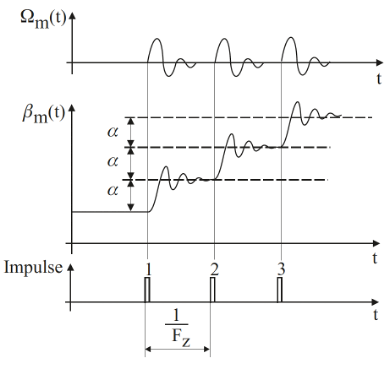
\includegraphics[width=8cm]{DiagrammVerlaufSchrittmotor.png}
		\caption{Zeitlicher Verlauf der mechanischen Winkelgeschwindigkeit und des Verdrehwinkels in Folge eines elektrischen Impulses in einer Statorwicklung (hier: VR-Schrittmotor); \cite{kleinantriebe}, S.433}
		\label{pic:diagrammSchrittmotor}
	\end{center}
\end{figure}


Da der Verdrehwinkel $\beta$ ein ganzzahliges Vielfaches des Schrittwinkels $\alpha$ ist, wird eine diskrete Positionierung ohne zusätzliche Sensorik möglich. Diese Art der Positionsbestimmung ist nur möglich, solange das maximale Drehmoment des Schrittmotors nicht überschritten wird. Ist das Lastmoment zu hoch, kommt es zu Schrittervlusten oder gar zum Stillstand.   Für die Ansteuerung eines Schrittmotors wereden durch eine Steuerlogik Impulse erzeugt. Damit wird ein Leistungselektronik-Stellglied gesteuert, das die Statorwicklungen bestromt (vgl. \cite{kleinantriebe}, S. 432). \newline

Auf die folgenden Grundtypen von Schrittmotoren soll nachfolgend näher eingegangen werden:
\begin{itemize}
	\item Reluktanz-Schrittmotor (VR)
	\item Permanenterregert Schrittmotor (PM)
	\item Hybrid-Schrittmotor (HY)
\end{itemize}

\newpage
In \autoref{pic:schrittmotor} ist der Aufbau eines Schrittmotors dargestellt. 
\begin{figure}[h]
	\begin{center}
		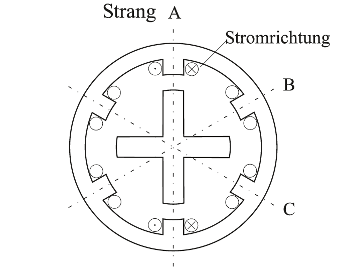
\includegraphics[width=6cm]{schrittmotor.png}
		\caption{Aufbau eines Schrittmotors (hier: VR-Schrittmotor); \cite{kleinantriebe}, S.432}
		\label{pic:schrittmotor}
	\end{center}
\end{figure}

\subsection{Der \acrshort{reluktanz}-Schrittmotor (VR)}

Beim \acrshort{reluktanz}-Schrittmotor ist der Rotor magnetisch und dessen Zahnteilung ungleich der Polteilung des Stators. Nach einem Umschalten des Statormagnetfeldes bewegt sich der in die sogenannte bis zum geringsten magnetischen Widerstand (Reluktanz). Diese Stellung wird auch als \acrshort{koinzidenzstellung} bezeichnet . 


\section{MQTT} %Acronym wieder einfuegen!
\acrshort{mqtt} ist ein Protokoll, welches zur digitalen Datenübertragung in ethernet-basierten Systemen dient. Es benötigt nur wenig Bandbreite und Ressourcen und verwendet eine 
Publish/Subscribe - Architektur. Das bedeutet, dass Nachrichten sogenannter Topics von Publishern bereitgestellt und von Subscribern empfangen werden. Der Datenverkehr wird über einen 
zentralen Broker verwaltet. Um die Publish Subscribe Architektur zu verstehen ist es hilfreich die Analogie zum Fernsehen zu bilden. Dabei senjdet ein TV-Sender sein Programm an einen bestimmten Kanal.
Auf diesen Kanal können nun beliebig viele Fernseher (Subscriber) zugreifen. Auch wenn keine aktive Verbindung zwischen Sender und Empfänger aufgebaut wird, erhalten beliebig viele Empfänger die benötigten Daten.
In \autoref{pic:mqttbroker} ist zu erkennen, wie die Daten nicht zwischen Publisher und Subscriber direkt, sondern über den zentralen Broker versendet werden. (Vgl. \cite{mqtt})

\begin{figure}[h]
    \begin{center}
        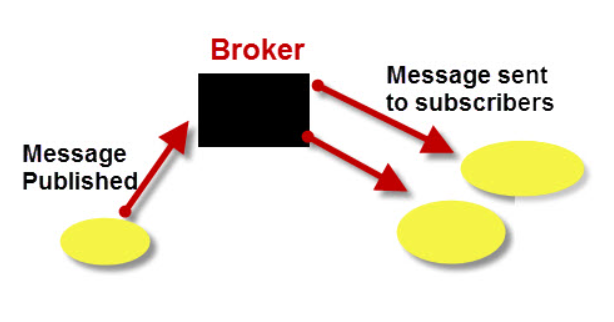
\includegraphics[width=8cm]{mqttbroker.png}
        \caption{\acrshort{mqtt}-Datenübertragung über den Broker}
        \label{pic:mqttbroker}
    \end{center}
\end{figure}
    \chapter{Anforderungsanalyse}
Der bisherige Aufbau der Gartenhochbahn soll verbessert und in einigen Bereichen erneuert werden. 
In diesem Kapitel wird mit Abschnitt \ref{sec:ausgangslage}
 zunächst das bisherige System beschrieben. 
Mit Abschnitt \ref{sec:anforderungen} folgen die resultierenden Anforderungen unterteilt in die jeweiligen Bereiche.  

\section{Ausgangslage}
\label{sec:ausgangslage}
Die Gartenhochbahn stellt ein Transportsystem dar. Hauptbestandteil des Systems ist eine Gondel, die sich über Laufräder 
auf einer Schiene fortbewegt. 

Der Antrieb der Gondel erfolgt durch einem Gleichstrommotor, der über \acrfull{pwm} angesteuert wird. Für die Bereitstellung der Energie ist eine Batterie in der Gondel installiert. Diese wird in der Parkstellung am Ende der Schiene aufgeladen. Als Abschaltung des Motors an den hinteren Endlagen sind Tastsensoren verbaut. Ein Read-Kontakt in der Gondel erkennt außerdem Magnete entlang der Strecke. Dadurch kann bereits vor Erreichen der Endlage die Geschwindigkeit reduziert werden. Für die Signalverarbeitung und Steuerung des Motors ist ein Arduino Nano im Einsatz. \\

Die Kraftübertragung des Motors auf das treibende Laufrad erfolgt bislang reibschlüssig. Das Getriebe weist dadurch einen hohen Verschleiß auf und ist nicht ausreichend zuverlässig. 

Durch die Sensorik ist eine Abschaltung bei Erreichen der Endlage möglich. Somit können einzelne Fahrzyklen der Hochbahn automatisiert durchgführt werden. 



\section{Anforderungen}
\label{sec:anforderungen}
\subsection{Antrieb}
Insgesamt soll der Antrieb eine hohe Verfügbarkeit aufweisen und verschleißarm sein. 
Die Kraftübertragung soll mit einer passenden Übersetzung erfolgen. Durch den elektrischen Motor soll eine Regelung der Geschwindigkeit und Drehrichtung möglich sein. Wünschenswert wäre außerdem eine Rückmeldung der Umdrehungen. 
Das Prinzipder Energieversorgung über eine Batterie soll beibehalten bleiben. 

\subsection{Bestellsystem}


Das Bestellsystem soll es Nutzern ermöglichen, die Hochbahn von der Terrasse aus mit einem Bestellauftrag zur Küche zu schicken. 
Dort soll ein Tablet die aktuelle Bestellung anzeigen. Ist alles für den Transport vorbereitet, kann ein Nutzer aus der Küche den Auftrag 
bestätigen und die Bahn fährt zur gewünschten Position zurück. Ein Webserver soll diese Funktionen über ein benutzerfreundliches \acrfull{gui} bereitstellen, welches über beliebige Engeräte ( z.B. Samrtphone oder Tablet) erreichbar ist.
Zudem soll die Möglichkeit bestehen, den Bestand zu erfassen. Das System soll selbstorganisierend sein, sodass sich auch das Kontingent durch Bestellungen aktualisiert. Dadurch soll verhindert werden, dass mehr bestellt werden kann als vorhanden ist.
Ebenfalls sollen Nutzer, die etwas bestellt haben, den aktuellen Lieferzustand einsehen können. D. h. es soll angezeigt werden, wo sich die Bahn befindet und welche Bestellung gerade bearbeitet wird.



\subsection{Sensorik}
Die erforderliche Sensorik kann in zwei Bereiche gegliedert werden: 

\begin{itemize}
	\item [a)] Positionserkennung 
	\item [b)] Kollisionsvermeidung  
	
\end{itemize}

Die Positionserkennung soll entlang der Strecke erfolgen. Die Information soll der Steuerung zur Verfügung gestellt werden. Dabei sollend die Positionswerte so exakt wie nötig ermittelt werden.

Die Kollisionsvermeidung soll Hindernisse im Fahrweg der Gondel erkennen und dadurch einen rechtzeitigen Stillstand gewährleisten. Dafür muss die Sensorik den kritischen Bereich ausreichend prüfen. 



\chapter{Vorgehensweise}
\label{sec:vorgehensweise}
In diesem Kapitel wird die Vorgehensweise zur Bewerkstelligung des Projektzieles beschrieben. Um das Ziel zu erreichen, stand zunächst die die Projektorganisation im Vordergrund. Diese wird im  \autoref{sec:projektorganisation} erläutert. 

\section{Projektorganisation}
\label{sec:projektorganisation}
Die Projektorganisation erfolgte anhand der folgenden Stufen: 

\begin{enumerate}
	\item Projektstrukturplan %Akronym erstellen PSD!
	\item Projektablaufplan 
	\item Kanban
	
\end{enumerate}

In einem ersten Schritt wurden mithilfe eines Projektstrukturplans die Teilbereiche definiert. Dadurch stellten sich die Wirkzusammenhänge der Bereiche heraus. Nachfolgend wurden die zugehörigen Aufgaben erstellt. Durch die Übersicht in einer Roadmap wurden die Aufgaben in einen zeitlichen Zusammenhang gebracht. 
In einem letzten Schritt folgte das Definieren der Aufgaben in einem Kanban-Board. 


\newpage
\subsection{Projektstrukturplan}
In \autoref{pic:structuremech} ist der  Projektstrukturplan mit den mechatronischen Komponenten dargestellt. 

\begin{figure}[h]
	\begin{center}
		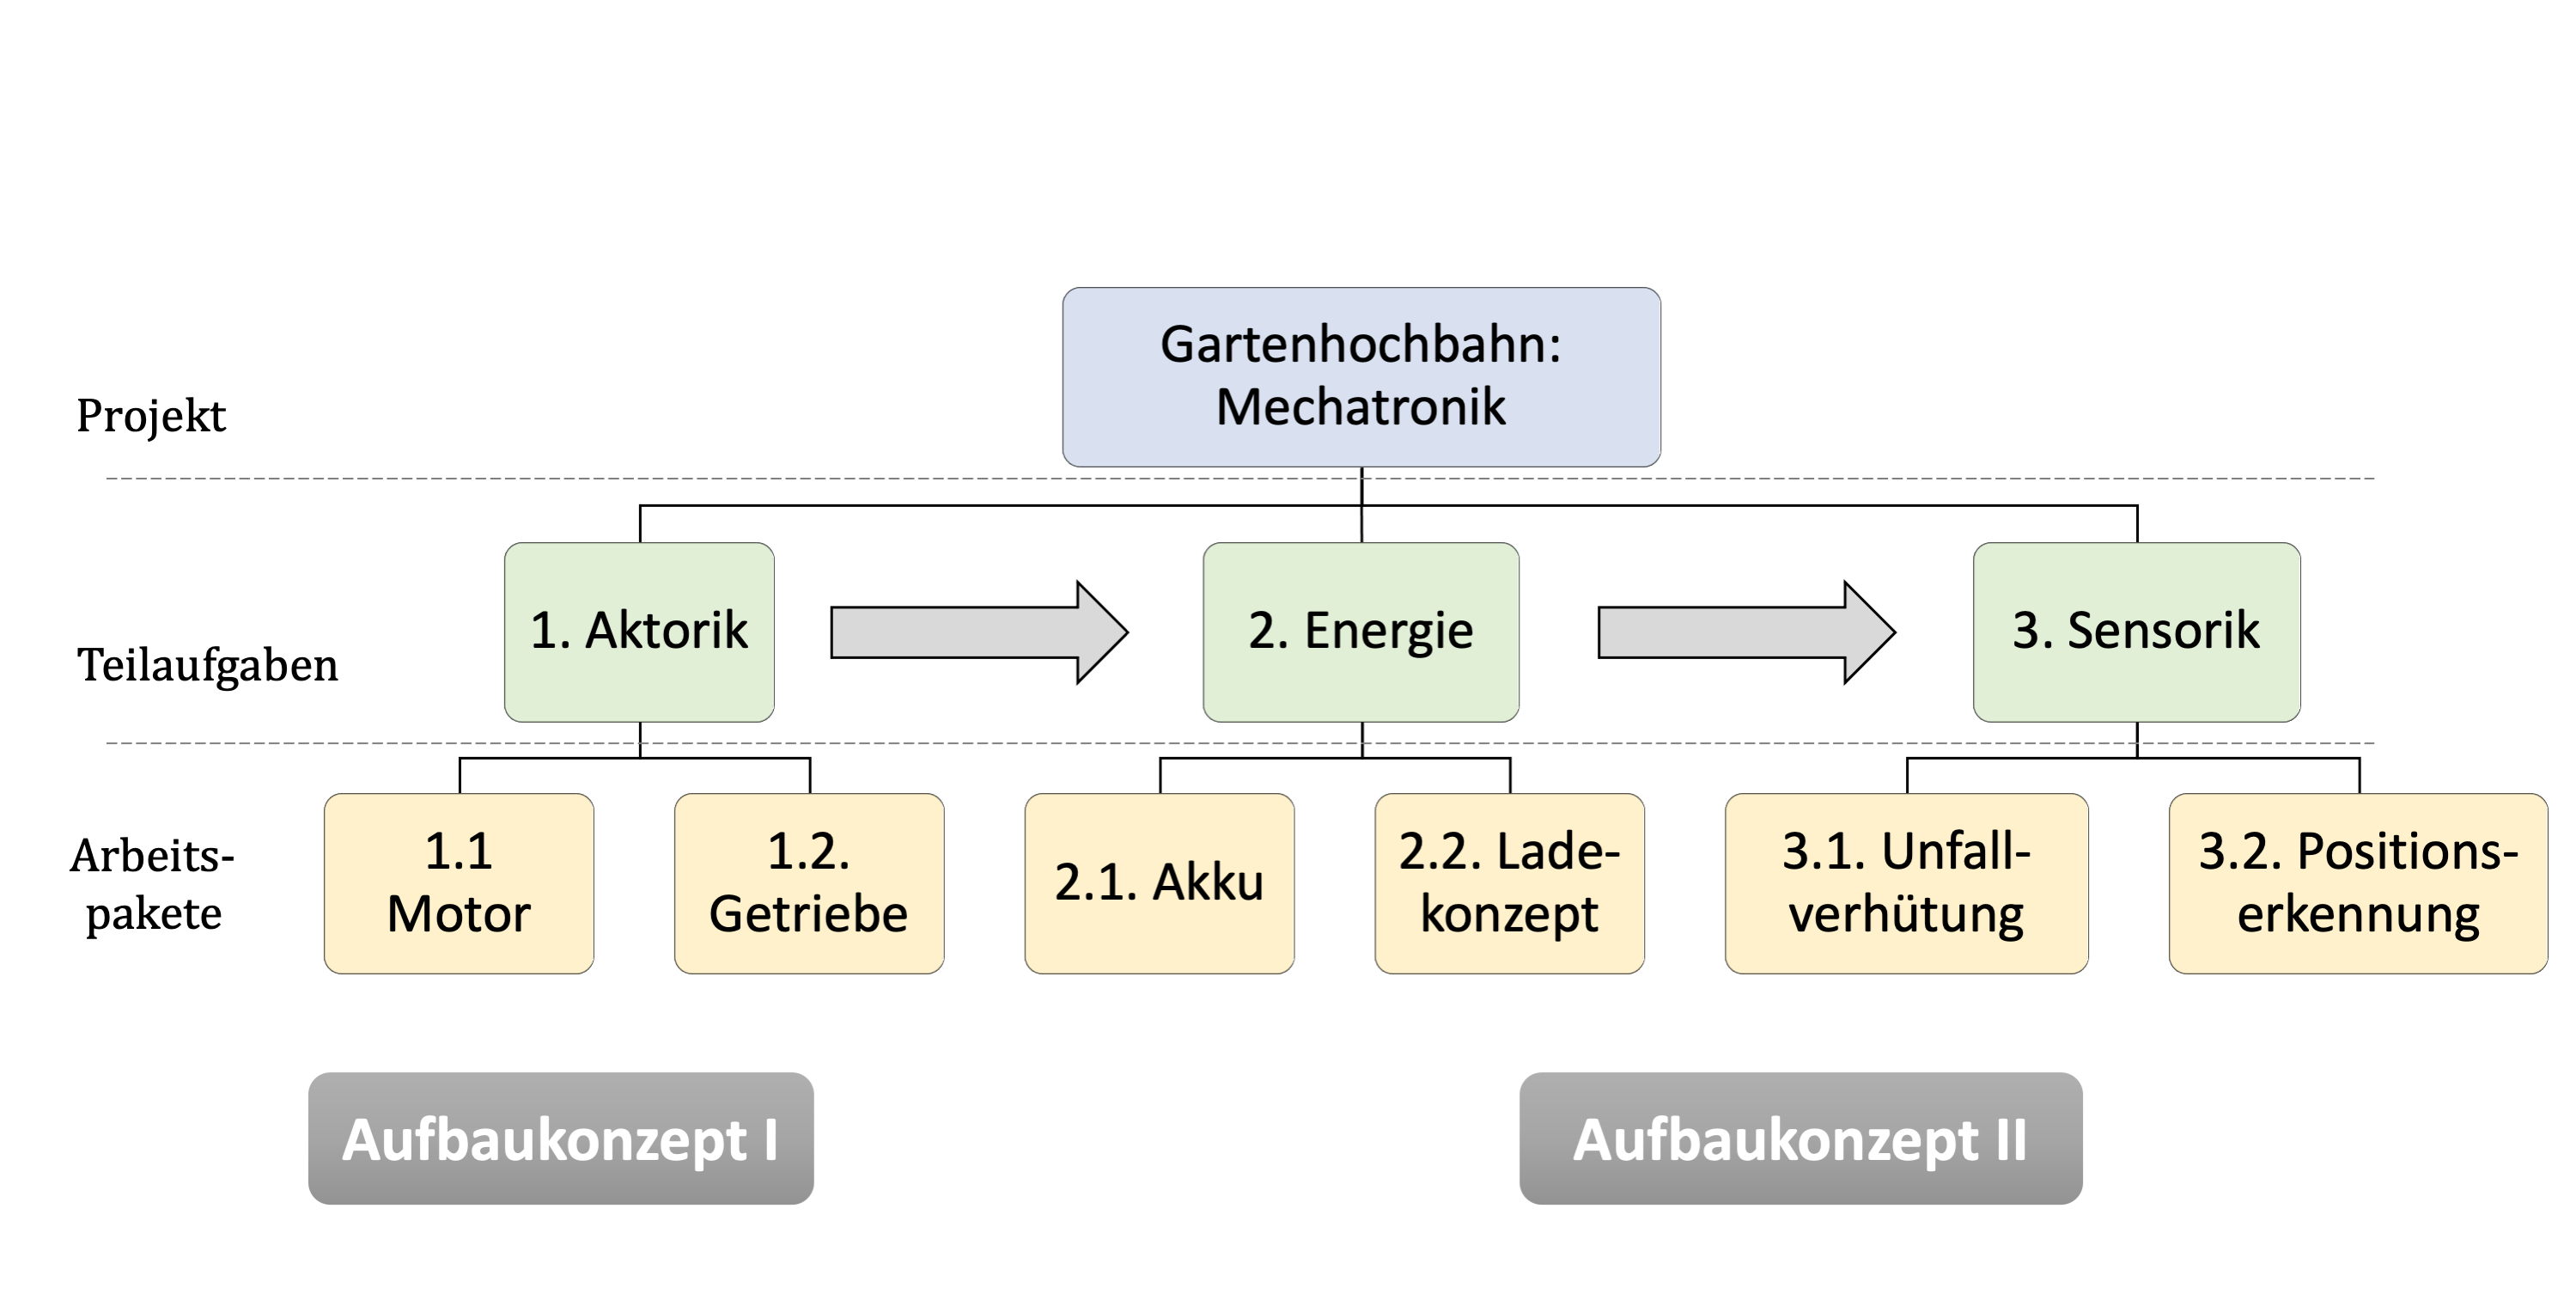
\includegraphics[width=17cm]{structureMech.png}
		\caption{Projektstrukturplan mechatronischer Komponenten}
		\label{pic:structuremech}
	\end{center}
\end{figure}

Das Projekt ist unterglieder in drei Teilaufgaben. Diese werden in der nächsten Ebene in Arbeitspakete untergliedert. 
Da die Bereiche aufeinander aufbauend sind, können Zusammenhänge analysiert werden. In dem Schaubild sind die Bereiche entsprechend der zeitlichen Abfolge aufgetragen. Dementsprechend soll in einem ersten Schritt die Aktorik konzeptioniert werden. Dazu zählt die elektrische und mechanische Komponente des Antriebs. Dieser erste Entwurf des Antriebs wird im Aufbaukonzept I festgehalten. Mit den elektrischen Leistungsdaten der Aktorik wird im nächten Schritt das Energiekonzept ausgearbeitet. Auf diesen Bereich baut final die Konzeptionierungsphase der Sensorik auf. \\ 
Durch weitere Anforderungen aus den Bereichen Energie und Sensorik folgt das Aufbaukonzept II. 

\newpage
\subsection{Projektablaufplan}
\label{projektablaufplan}
 %Wird noch schön eingefügt, fürs Testat reichts erst mal. 
%Werden auch in einem zweiten Schritt diene Aufgaben einfügen. 
Aus dem Projektstrukturplan geht der Projektablaufplan hervor. Darin werden die zuvor definierten Arbeitspakete aus den Teilaufgaben terminiert. 
\begin{figure}[h]
	\begin{center}
		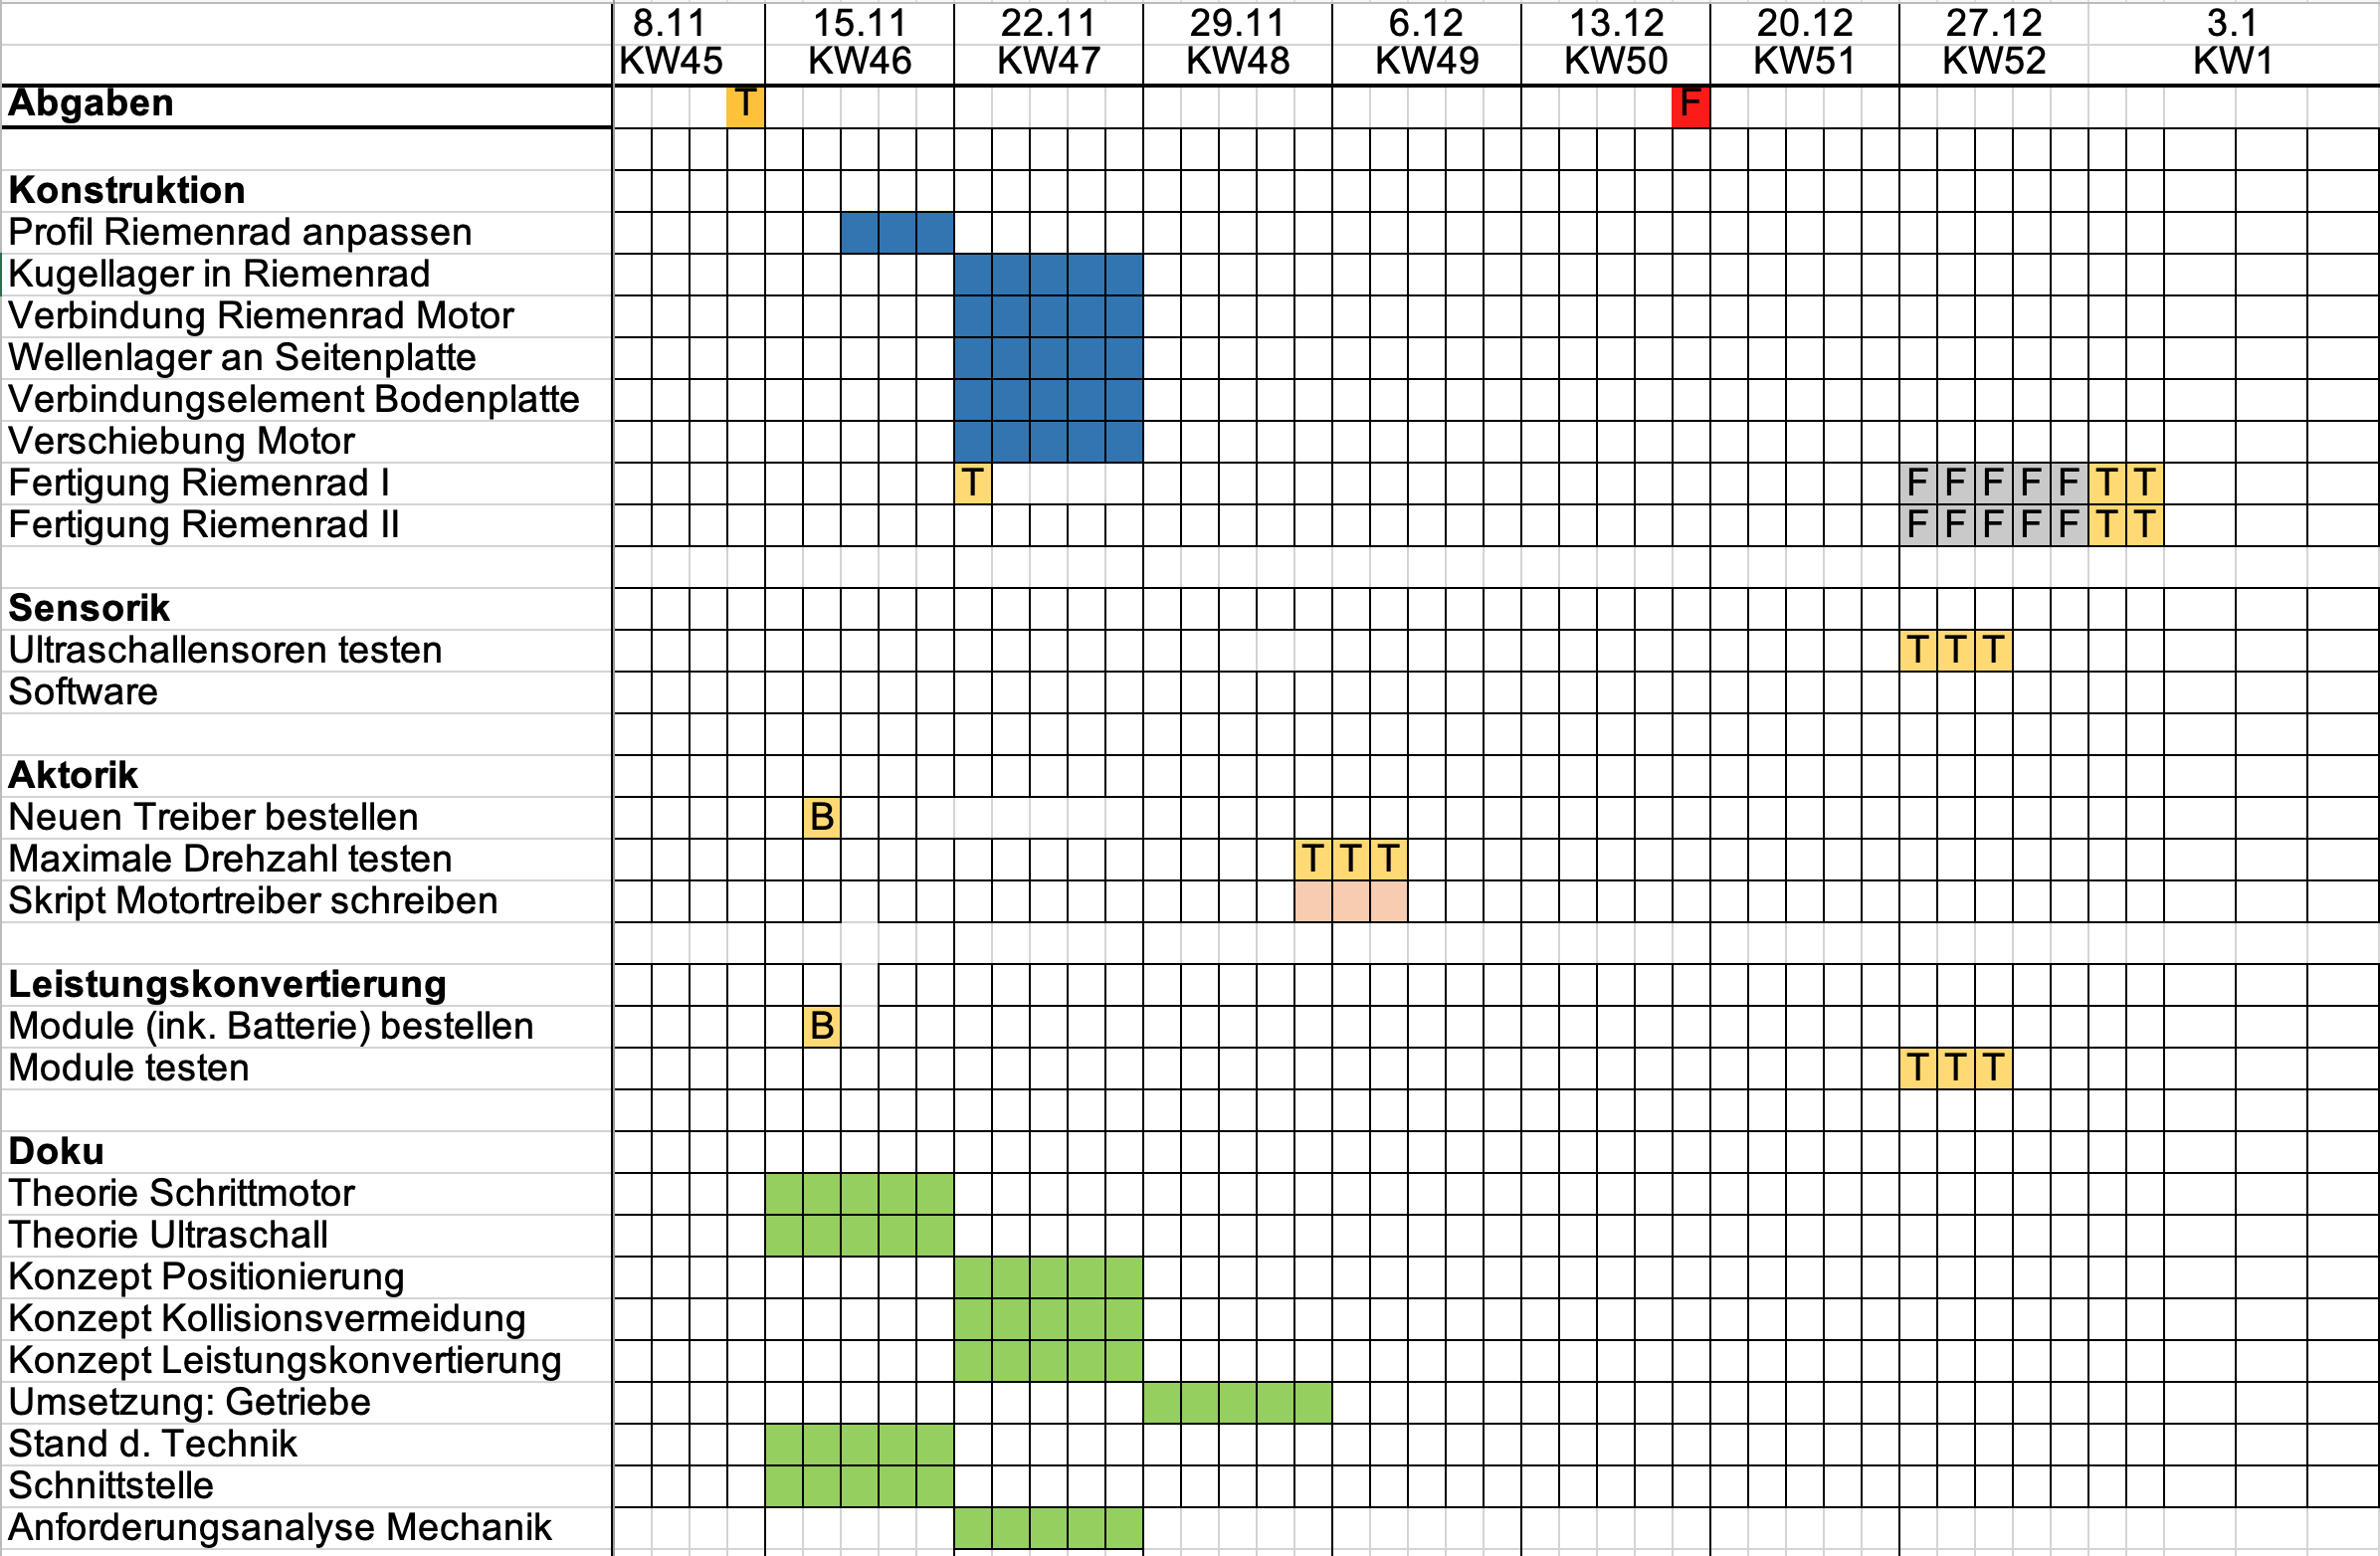
\includegraphics[width=17cm]{roadmap.png}
		\caption{Projaktablaufplan mechatronischer Komponenten}
		\label{pic:roadmap}
	\end{center}
\end{figure}



\newpage
\subsection{Arbeitsmangement}
\label{sec:arbeitsmanagement}
Für das Arbeitsmanagement wird die Kanban-Methode verwendet. Dabei werden die Teilaufgaben dem Bearebeitungsstatus zugeordnet. Im Rahmen des Projektes wurden die Stati \textit{Backlog}, \textit{Todo,  In Progress, Testing} und \textit{Done}  unterschieden. Die Aufgaben wurden mit den Berbeitungszeiträume aus dem Projektablaufplan definiert und dem entsprechenden Bearbeiter zugewiesen. 	
Für die Kanban-Methode kam das Tool "trello" zum Einsatz. Ein Bildausschnitt aus dem Kanban-Board ist in \autoref{pic:kanban} dargestellt. 


\begin{figure}[h] %Würde ich evtl. in finaler Abgabe raus lassen!
	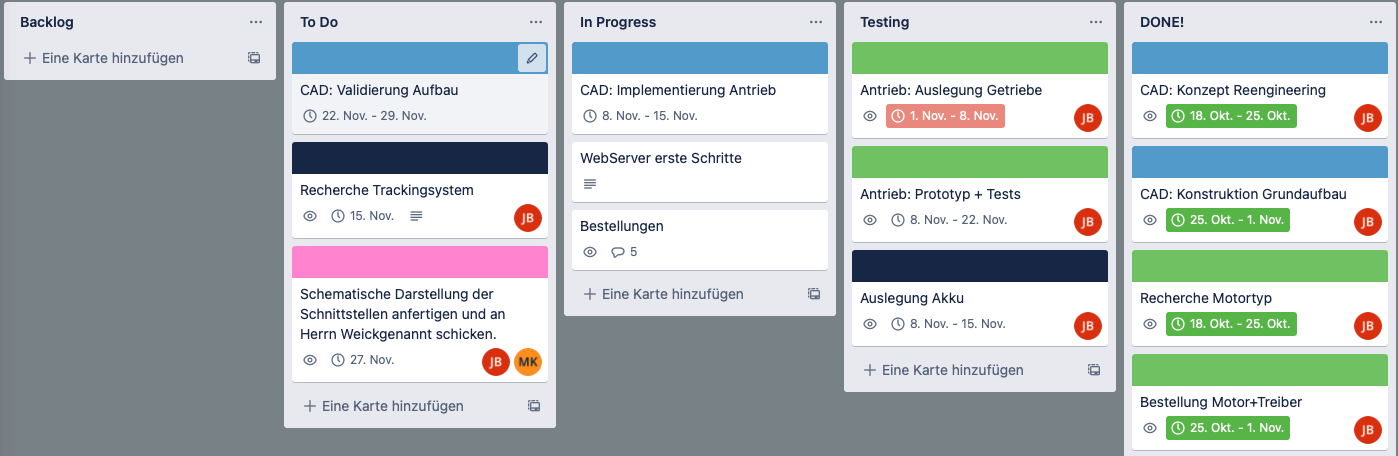
\includegraphics[width=17cm]{kanban.png}
	\caption{Bildausschnitt aus dem Kanban-Board}
	\label{pic:kanban}
\end{figure}


\chapter{Konzept}
Aufgrund der gestellten Anforderungen werden in diesem Kapitel die Konzepte zum Erreichen der Teilaufgaben erläutert. \newpage

%ich wäre schon dafür, dass man keine neue Seite anfängt und das Bild in die Mitte setzt... 
%Nur Latex sieht das vermutlich anders... 
\section{Grundaufbau}
\textcolor{red}{Platzhalter:Begründung, weshalb Neuaufbau nötig}\\
In  \autoref{pic:grundaufbau} ist das Konzept des Grundaufbaus der Gondel dargestellt. Dieser soll aus den beiden Baugruppen \textit{Triebwagen} und \textit{Stützwagen} bestehen. Im Triebwagen sind Motor und Getriebe verbaut. An die beiden Wägen anchließend werden nach unten Verbindungselemente für die Befestigung des Tabletts sowie für die Elektronik angebracht. \\
Die detaillierte Konzeptionierung der dargestellten Komponenten erfolgt in den nachfolgenden Abschnitten. 

\textbf{Fertigungsmethode} 

\begin{figure}[h]
	\centering
	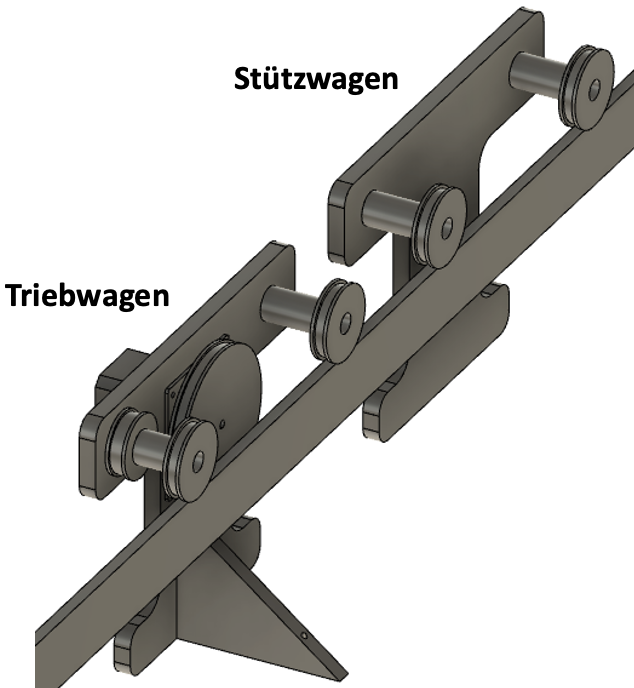
\includegraphics[width=10cm]{grundaufbau.png} 
	\caption{Grundaufbau von Trieb- und Stützwagen}
	\label{pic:grundaufbau}
\end{figure}

\begin{figure}[h]
	\centering
	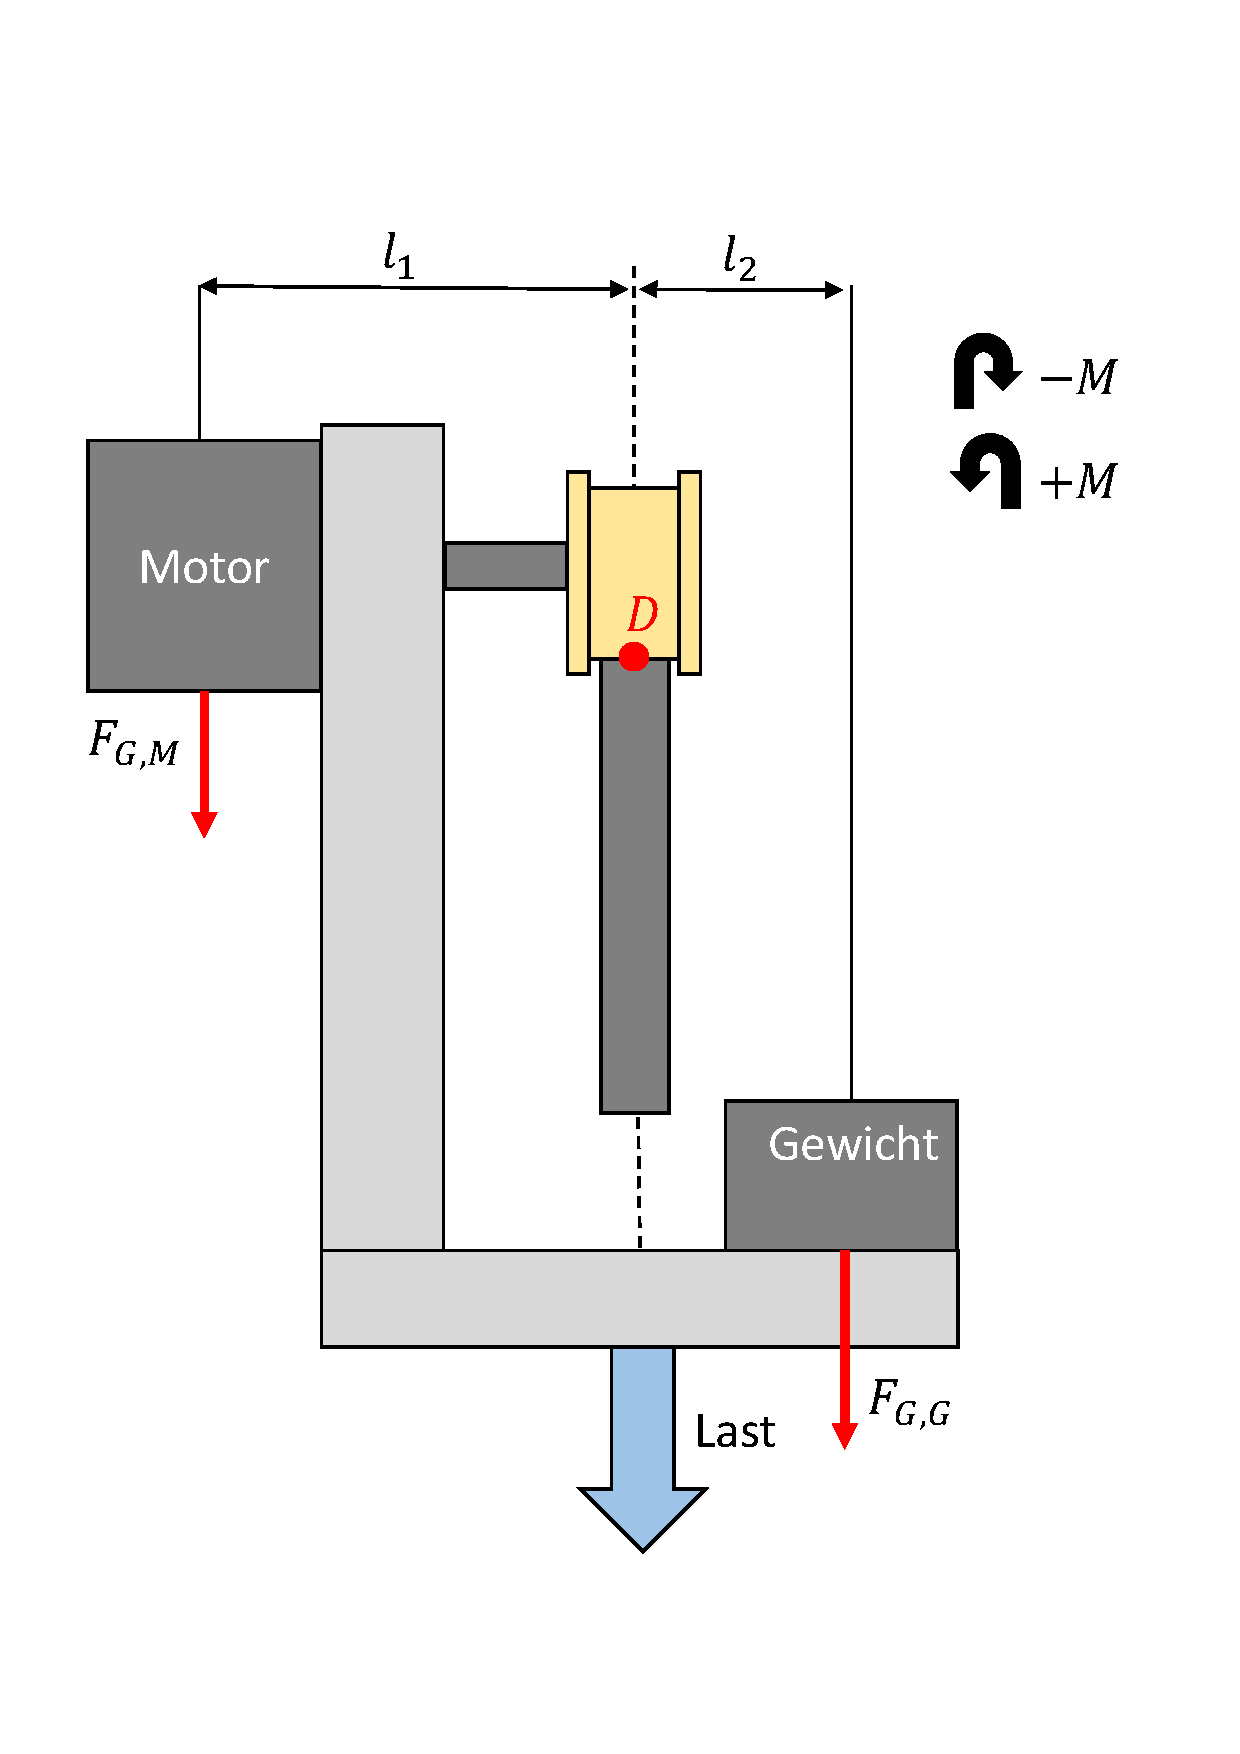
\includegraphics[width=10cm]{kippmoment.pdf} 
	\caption{Grundaufbau von Trieb- und Stützwagen}
	\label{pic:kippmoment}
\end{figure}




\section{Aktorik}
In diesem Abschnitt wird die Konzeptionierung des Antriebs der Gartenhochbahn beschrieben. In \autoref{sec:motor} wird zunächst die Auswahl und Auslegung des Motors beschrieben. Das Drehmoment des Motors soll anschließend auf ein Laufrad übertragen werden. Die Beschreibung des dafür zuständigen Getriebes folgt mit \autoref{sec:getriebekonzept}

\subsection{Motor}
\label{sec:motor}
Für den Antrieb der Gartenhochbahn wurde zwischen einem DC-Motor und einem Schrittmotor ausgewählt. 
Bei einem DC-Motor wird das Signal zur Steuerung der Drehzahl vom Arduino mit PWM an einen Motortreiber übermittelt. Dieser ist für die Leistungsübersetzung des Signals und die Implementierung der Richtungsumkehr zuständig. 

Bei der Steuerung eines Schrittmotors werden von einem Treiber positive Taktflanken ausgewertet. Bei jeder Taktflanke erfolgt eine Umpolung der Spulen in der Art, dass sich ein Inkrementalschritt ergibt. Umgekehrt können aufgrund der erzeugten Taktflanken Rückschlüsse auf die Umdrehungen des Motors und somit auf die Wegstrecke gemacht werden. 

Diese Information kann für die Positionsbestimmung der Gartenhochbahn genutzt werden. Aus diesem Grund soll für den Antrieb ein Schrittmotor verwendet werden. Dafür kommt der Motor Nema 17-04 von Joy-IT zum Einsatz. Als Schrittmotortreiber wird der DRV8825 von Texas Instruments verwendet. 



\subsection{Getriebe}
\label{sec:getriebekonzept}
Das Getriebe sorgt für die Kraftübertragung des Motordrehmoments auf die Schiene. Zusätzlich ist die Geschwindigkeit der Hochbahn vom Übersetzungsverhältnis des Getriebes abhängig. Nachfolgend wird die Auswahl der Getriebeart und anschließend die Auslegung beschrieben. \\

\underline{Getriebeart}\\
Für die Auswahl der Getriebe steht ein Zahnradgetriebe und ein Zugmittelgetriebe im Raum. Das Zahnradgetriebe besitzt eine formschlüssige Kraftübertragung der beiden Räder. Damit diese mit dem geeigneten Kopfspiel zustande kommt, müssen die beiden Wellen in einem exakten Abstand zueinander stehen. Das bedarf einem hohen Grad an Präzision bei der Fertigung. Bei einem Zugmittelgetriebe kann eine Spannrolle dafür sorgen, dass das Zugmittel ausreichend gespannt ist. Dadurch muss der Abstand der beiden Räder zueinander ein niedrigeres Maß an Genauigkeit besitzen. 
Für das Projekt wird ein Zugmittelgetriebe verwendet. Um dabei Schlupf zu vermeiden, wird ein T-Profil bei Riemen und Rad verwendet. 
\\


\underline{Konstruktion und Fertigung}\\
Der Antrieb besteht aus den folgenden Komponenten: getriebenes- und treibendes Riemenrad, Laufrad und Zahnriemen. Zunächst wird das Konzept für das getriebene Riemenrad und das Laufrad beschrieben. Anschließend erfolgt die Beschreibung des gesamten Antriebs anhand der Konstruktion.  

Das Laufrad kommt für den Abtrieb auf der Schiene zum Einsatz. Eine Herausforderung stellt dabei die Kraftübertragung vom Laufrad auf das getriebene Riemenrade dar. Dazu wurden zwei Konzept entwickelt. Die Gegenüberstellung ist in \autoref{pic:abtriebkonzepte} dargestellt.

\begin{figure}[h]
	\begin{center}
		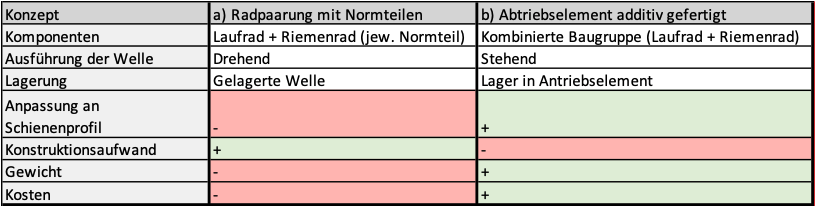
\includegraphics[width=17cm]{abtriebkonzepte.png}
		\caption{Konzepte für die Kraftübertragung von Riemenrad auf das Laufrad}
		\label{pic:abtriebkonzepte}
	\end{center}
\end{figure}
\newpage
Bei Konzept a) wird für  Laufrad und Riemenrad jeweils ein Normteil verwendet. Die Kraftübertragung zwischen den beiden Rädern erfolgt über eine Welle. Diese ist gelagert während die beiden Räder stehend auf der Welle montiert sind.
Bei Konzept b) handelt es sich um eine Baugruppe, bestehend aus Laufrad und Riemenrad. Das kombinierte Bauteil wird additiv gefertigt. Es ist stehend auf der Welle gelagert.  Die Welle selbst ist stehend ausgeführt. 
Durch die additive Fertigung muss eine Konstruktion des Bauteils erfolgen. Dadurch ergibt sich in diesem Punkt ein höherer Aufwand als bei der Verwendung von Normteilen. Die Konstruktion bietet jedoch den Vorteil, dass das Laufrad an das Profil der Schiene angepasst werden kann. Die Normteile der beiden Räder sind meist für hohe Krafteinwirkungen in industriellem Einsatz ausgelegt. Dadurch ergibt sich bei Verwendung der Räder ein hohes Gewicht. Zusätzlich sind die Bauteile mit hohen Kosten verbunden. Die additive Fertigung des Bauteils sollte für die Krafteinwirkung ausreichend sein. Aufgrund der genannten Vorteile kommt für das Projekt Konzept b) zum Einsatz.  

\newpage

\section{Energieversorgung}
Die Batterie dient als Energieversorgung für Aktorik, Sensorik und Steuerung. Um für die Komponenten passende Ströme und Spannungen bereitstellen zu können, ist eine Leitsungskonvertierung notwendig. In \autoref{pic:leistungskonvertierung} sind die diesem Zweck verwendeten Komponenten dargestellt und in \autoref{tbl:leistungskonvertierung} aufgelistet. 

\begin{figure}[h]
	\begin{center}
		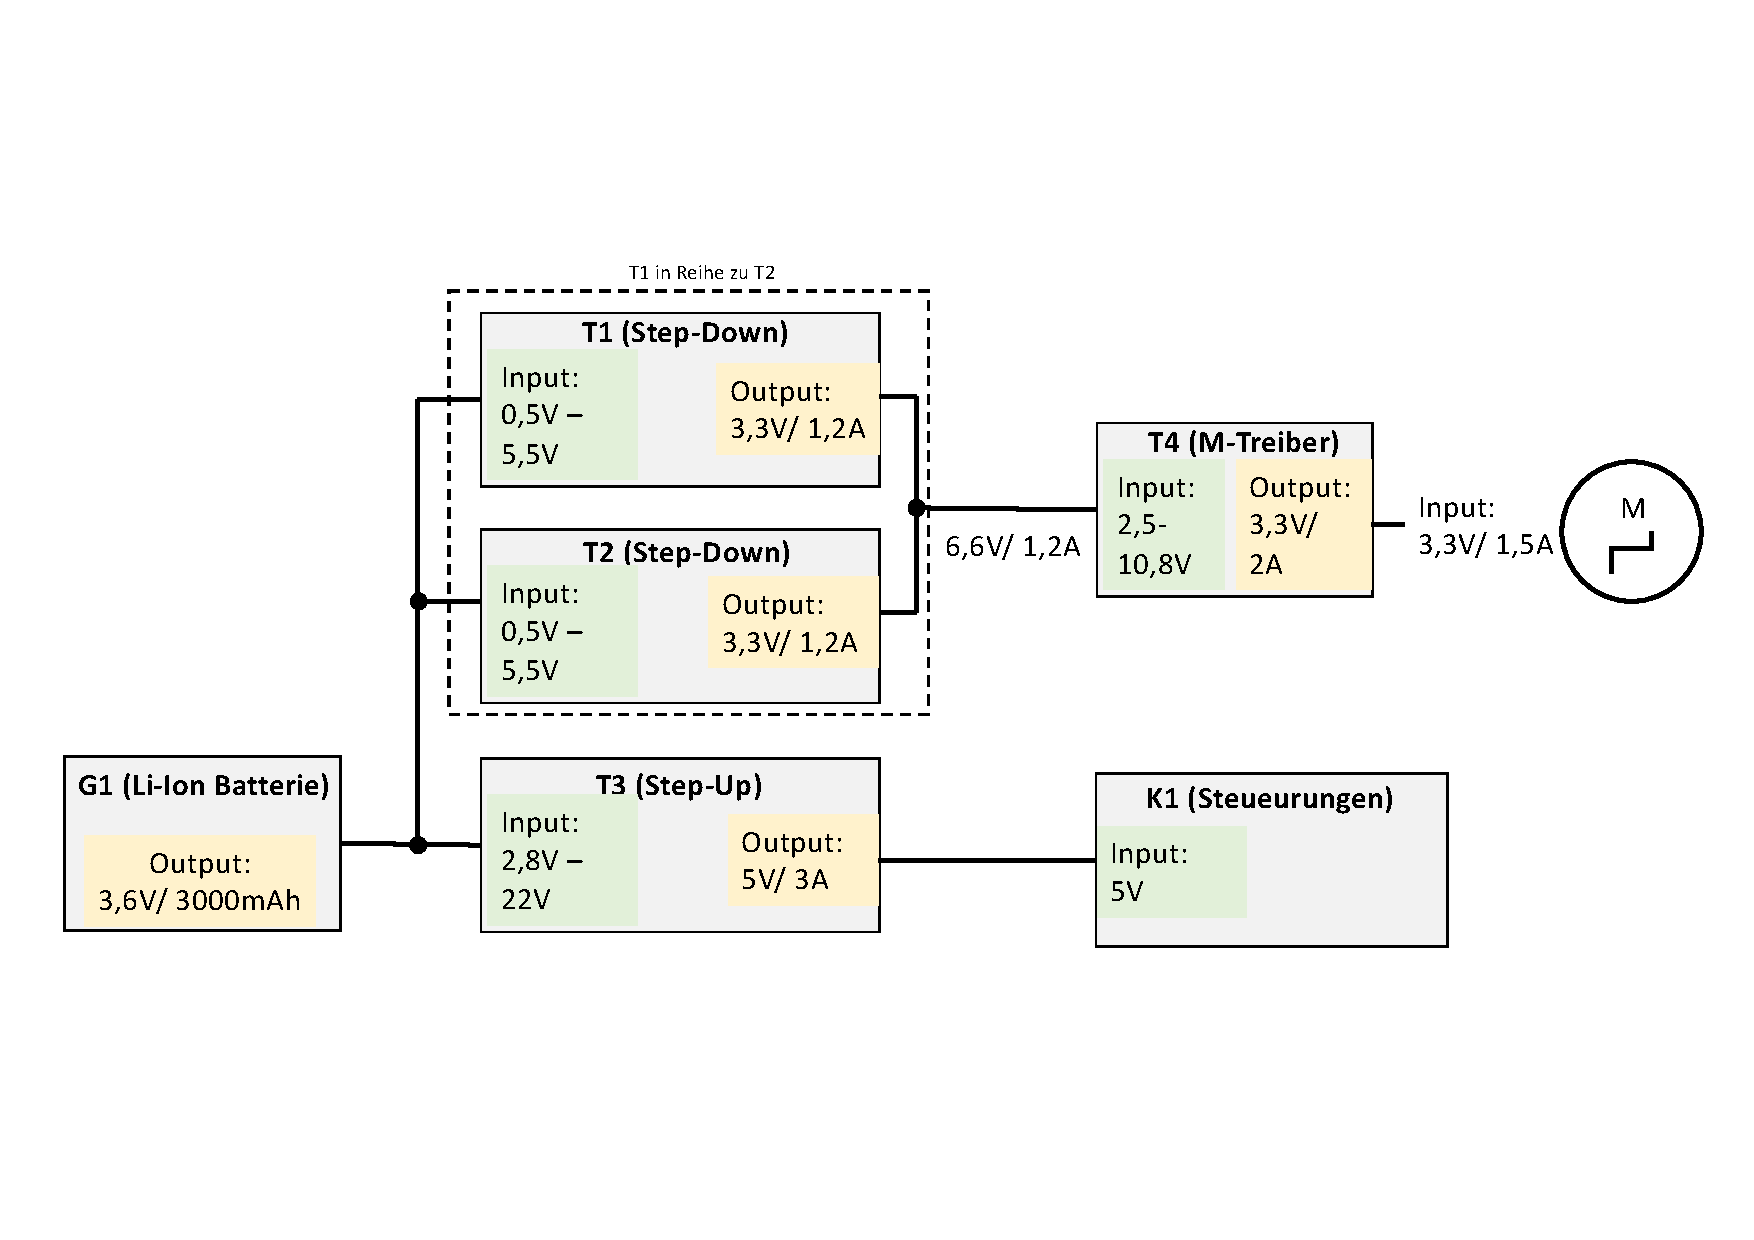
\includegraphics[width=15cm]{leistungskonvertierung.pdf}
		\caption{Schema zur Leistungskonvertierung der elektrischen Komponenten}
		\label{pic:leistungskonvertierung}
	\end{center}
\end{figure}


\begin{table}
	\begin{center}
		\begin{tabular}[h]{l|l|l}
			\textbf{Name} & \textbf{Bezeichnung} & \textbf{Bauteill}\\
			\hline
			G1 & Li-Ion Batterie & Panasonic NCR18650B\\
			\hline
			T1-T2 & Step-Down Converter & Polulu S13V30F5\\
			\hline
			T3 & Step-Up Converter & Polulu U1V11F3\\
			\hline
			T4 & Schrittmotor Treiber & Polulu DRV8834 \\
			\hline
			K1 & Steueurungen & Arduino Nano, ESP32 \\
		\end{tabular}
	\end{center}
	\caption{Bezeichnungen verwendeter Komponenten}
	\label{tbl:leistungskonvertierung}
\end{table}

Die Li-Ion Batterie darf eine minimale Zellspannung $U_{min} =2,75V$ nicht unterschreiten. Zu diesem Zweck lässt sich die \acrshort{cutoffvoltage} bei den beiden Step-Down Convertern $T1$ und $T2$ einstellen. Damit wird bei  niedrigem Batteriezustand die Leistungselektronik abgeschaltet. Die Steuerung ist anschließend noch immer aktiv, sodass eine Kommunikation mit dem Hochbahncontroller weiterhin möglich bleibt. Die beiden Converter sind in Reihe geschalten um die erforderlichen Leistungen des Schrittmotors bereitstellen zu können. Am Schrittmotortreiber $T4$ lässt sich die für den Motor geforderte Spannung und der maximale Strom einstellen. Dafür findet im Treiber ebenfalls eine Leistungskonvertierung von $V_{in}=6,6V$ auf $V_{Motor}=3,3V$ statt. Der Step-Up Converter $T3$ passt die Eingangsspannung an die erforderliche Spannung der Controller an Die Ausgangsspannung des Converters liegt bei $5 \pm 0,15 V$ \\

Die Li-Ion Batterie soll in der Parkposition der Hochbahn aufgeladen werden. Die Batterie kann bei einer Ladespannung von $4,2V$ aufgeladen werden. Für die Steueurung des Ladevorgangs kommt der Ladecontroller MCP73831/2 von Microchip zum Einsatz. Der Controller lässt einen Ladestrom von 	$500mA$ zu. 


\newpage

\section{Sensorik}
\subsection{Kollisionsvermeidung}
Für die Kollisionsvermeidung soll mithilfe von Ultraschallsensoren kontinuierlich die Distanz $d$ zum nächsten Objekt gemessen werden. Als Sensor kommt der HC-SR04 auf dem Tablett angebracht. Der Messbereich beträgt $0,02m - 5m$ (\cite{hcrs04}). Die Kollisionsvermeidung soll anhand von einem Warn- und einem Schutzfeld geschehen. Das Warnfeld wird ausgelöst, wenn bei mindestens einem der beiden Sensoren $d<1,5m$ erfüllt ist. Eine Schutzfeldverletzung erfolgt bei $d<0,7m$. Die Breite $b$ des kleinsten zu erfassende Objektes beim Öffnungswinkel $\alpha = 30°$ beträgt $b= tan(\alpha) \cdot d \cdot 2$. Dabei beträgt das kleinste erfassbare Objekt am Ende des Schutzfelds $b_S \approx 0,4m$ und am Ende des Warnfelds $b_W \approx 0,8m$. \\
In \autoref{pic:kollisionsvermeidung} sind die beiden Ultraschallsensoren sowie Warn- und Schutzfeld dargestellt. 

\begin{figure}[h]
	\begin{center}
		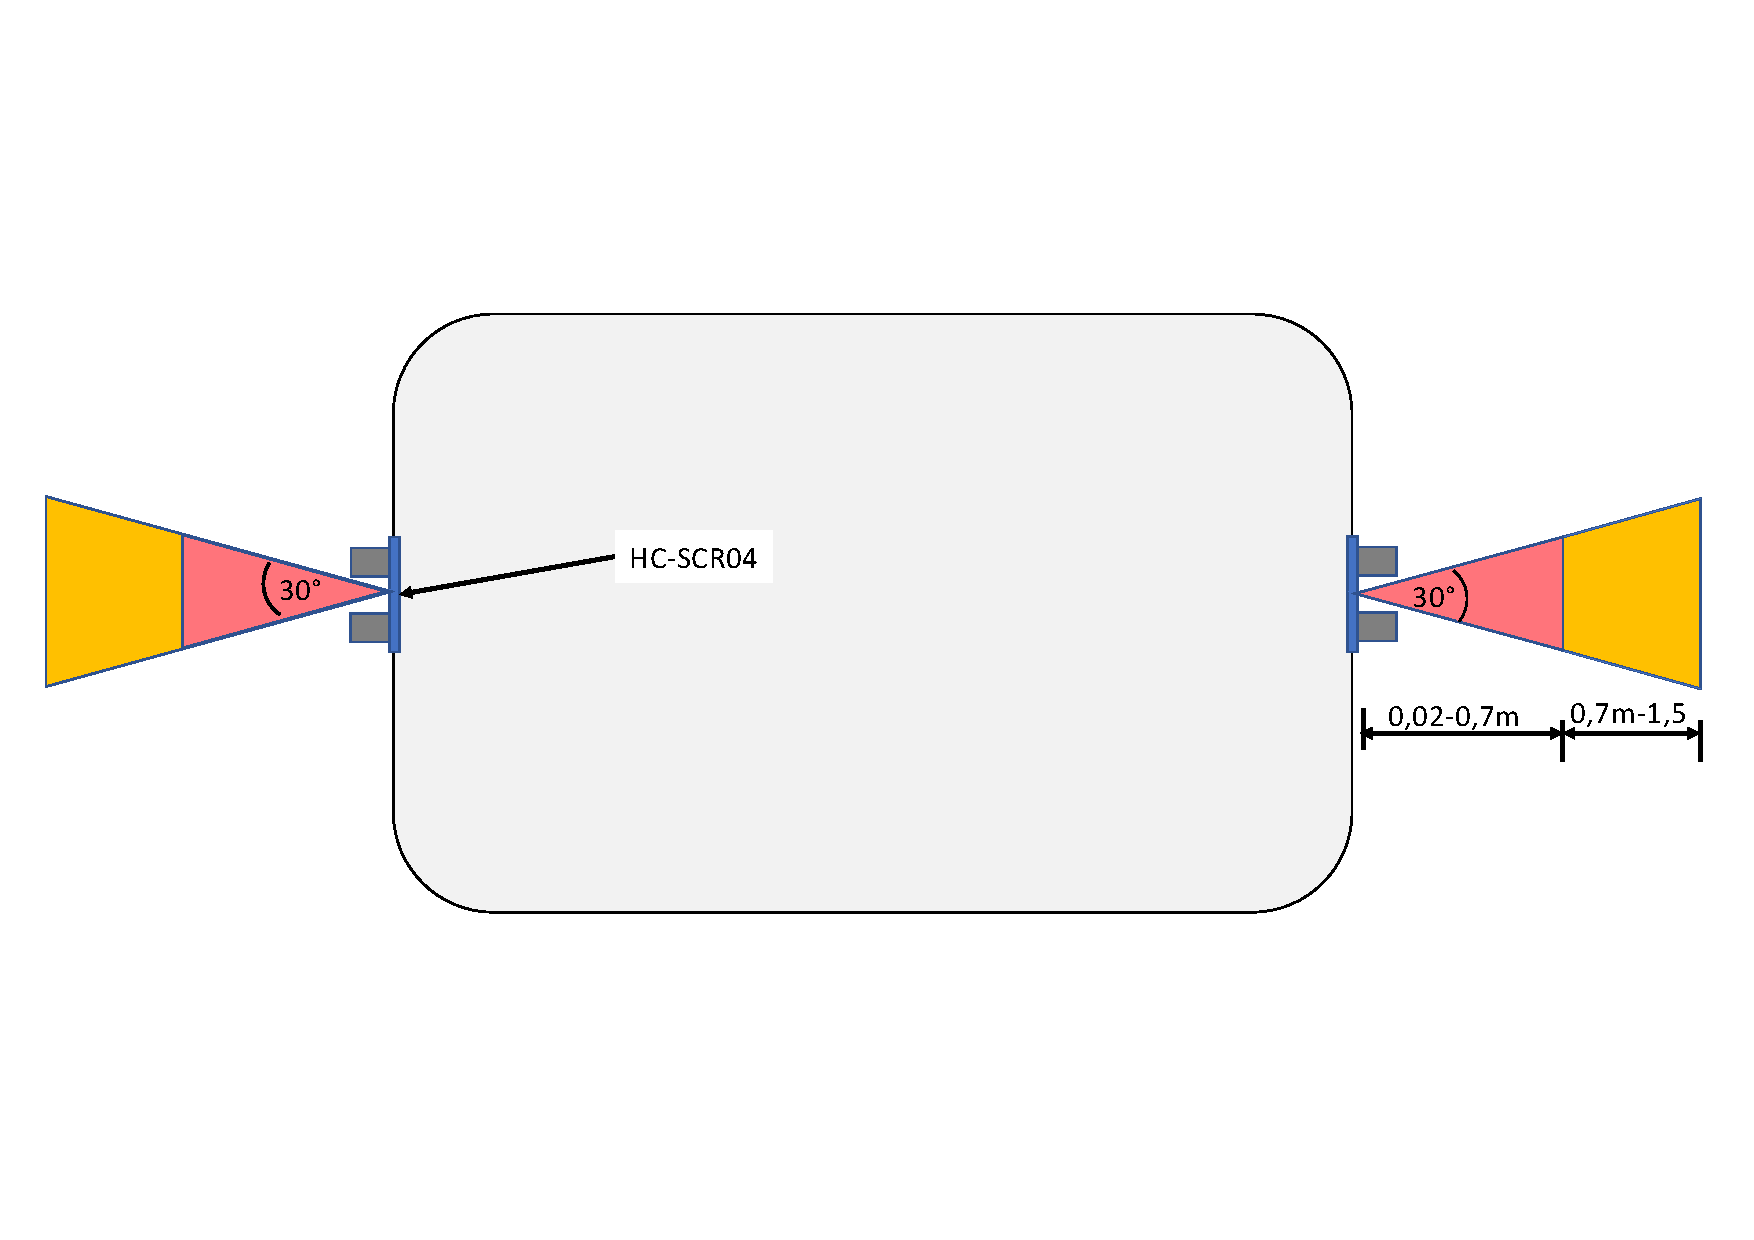
\includegraphics[width=15cm]{kollisionsvermeidung.pdf}
		\caption{Schematische Anordnung der Ultraschallsensoren HC-SR04 auf dem Tablett zur Kollisionsvermeidung}
		\label{pic:kollisionsvermeidung}
	\end{center}
\end{figure}

\newpage
Der Ultraschallsensor HC-SCR04 Ultraschallsensor verfügt für die Messung der Schalllaufzeit über die beiden Pins \textit{TRIG} und \textit{ECHO}. Die Messung wird durch eine fallende Flanke von 10µs am Triggereingang gestartet. Anschließend werden über den  Piezokristall des Sensors acht aufeinanderfolgende 40Khz Schallwellen ausgesandt. Nach diesen 200µs setzt der Sensor den \textit{ECHO} so lange auf high, bis der Ultraschallimpuls empfangen wurde. Wurde keine Schallreflektion empfangen, verbleibt der \textit{Echo} für max. 38 ms auf HIGH. Eine erneute Messung kann frühestens nach 20ms gestartet werden. (vgl. \cite{hcrs04})

Mit einem Arduino Nano werden die Messungen an beiden Sensoren zyklisch durchgeführt. Die Berechnung der Distanz erfolgt anhand der in \autoref{sec:ultraschall} beschriebenen Formel. Tritt eine Schutz- oder Warnfeldverletzung auf, gibt der Arduino ein Signal auf einen entsprechenden Interrupt-Pin am ESP32 als  Hochbahn-Controller. Die verwendeten Interupt-Pins sind nachfolgend dargestellt. \\


\begin{center}
	\begin{tabular}[h]{l|l|l}
		Sensor & Verletzung  & ESP32 Interrupt-Pin \\
		\hline
		1 & Warnfeld & GPIO1\\
		\hline
		1 & Schutzfeld & GPIO2\\
		\hline
		2 & Warnfeld & GPIO3\\
		\hline
		2 & Schutzfeld & GPIO4\\	
	\end{tabular}
\end{center}


\subsection{Positionserfassung}
\newpage
\section{Schnittstelle}
Als Übergang von der Konzeptionierung mechatronischer Komponente zu den informationstechnischen Konzepten soll in diesem Abschnitt die Schnittstelle aller verwendeten Komponenten vorgestellt werden. Dazu ist in \autoref{pic:schnittstellen} eine Übersicht dargestellt.

\begin{figure}[h]
	\centering
	\includegraphics[width=17cm]{schnittstellen.pdf}
	\caption{Schnittstellenübersicht der verwendeteter Komponenten}
	\label{pic:schnittstellen}
\end{figure}

%@Moritz: Hoffe, es passt so für dich. Kannst gerne alles auch wieder anders schreiben ;) Habe aber eig alles von dir drinne  und nur ergänzt... 

In der Übersicht sind die Komponenten hierarchisch dargestellt. Die Pfeile dazwischen stellen die Schnittstellen dar. Der Webserver kommuniziert mit den Endgeräten der Kunden oder dem Tablet in der Küche über \acrshort{http}. Mit POST-Requests werden Steuerbefehle oder Bestellungen zur weiteren Verarbeitung an den Server geschickt.
\acrshort{mqtt} dient zur Kommunikation zwischen dem Server und Hochbahn. Für die Übermittlung der \acrshort{mqtt}-Befehle  befindet sich ein \acrshort{mqttBroker} auf der Kommunikationsebene. Die Hochbahn bekommt Information über die Station, die angefahren werden soll. Während der Fahrt gibt die Bahn Rückmeldung über die aktuelle Position. Außerdem sollen Kollisionswarnungen übertragen werden. Auf der Hochbahn führt ein D1-Mini als Controller die Kommunikation durch. Dieser steuert außerdem die beiden Steuerungen für den Motor und der Kollisionsvermeidung. Für die beiden ausgelagerten Steuerungen werden jeweils Arduino Nanos verwendet. Die Motorsteuerung empfängt die Befehle zur gewünschten Motordrehzahl. Aus den Befehlen werden die benötigten Takte für den Schrittmotortreiber generiert. Die Sicherheitssteuerung überprüft kontinuierlich die Distanzwerte der Ultraschallesnsoren. Ist eine Kollision zu erwarten, setzt die Steuerung einen Interrupt des Hochbahn-Controllers. Zwischen D1-Mini und Motor-Arduino wird über die RX und TX - Pins eine serielle Kommunikationsschnittstelle aufgebaut, während der Arduino zur Kollisionsvorbeugung direkt an Interrupt Pins. Dadurch erlangen die Signale höchste Priorität und die Steuerung kann somit schnell reagieren. Die Positionserfassung wird vom Hochbahn-Controller anhand der Schaltvorgänge des Reed-Kontaktes und der aktuellen Motordrehzahl berechnet. \newpage

\section{Software}
Es gibt in diesem Projekt zwei Hauptsoftwarekomponenten, welche die Anlage steuern: Der Server, welcher Anfragen und Befehle an die Bahn verwaltet und die Bahn selbst,
welche für die Steuerung der Hardware zuständig ist. Der Server soll im Heimnetzwerk über die Adresse des Hosting-System erreichbar sein. Befehle an die Hochbahn sollen drahtlos mit \acrshort{mqtt} übertragen werden.
Auf der Bahn kommuniziert ein Arduino über einen ESP8266 mit dem Server und steuert gleichzeitig die Bahn. In den folgeneden Abschnitten wird die Konzeption dieser einzelnen Softwareteilen erläutert.

\subsection{Web-Applikation}
Die Web-Applikation bezeichnet die Benutzeroberfläche, welche sowohl in der Küche zum Einsehen von Bestellungen, als auch von Gästen zum Bestellen und Steuern der Bahn verwendet wird. Jeder Gast soll sich ein Konto erstellen und dabei seine Lieblingsfarbe auswählen können.
Bestellt dieser etwas kann so die Hochbahn in der individuellen Farbe leuchten. Dies dient zum einen der Freude der Gäste und zum anderen zum Erkennen, für wen die Bestellung ist. Angemeldet soll ein Nutzer über ein Menü unter folgenden Optionen
wählen können:
\begin{itemize}
	\item Allgemeines
	\item Mein Konto
	\item Bestellen
	\item Steuern
	\item Live-Verfolgung
\end{itemize}
Unter \textit{Allgemeines} werden generelle Infos zur Hochbahn angezeigt. Kontoeinstellungen wie Änderung der E-Mail Adresse oder Lieblingsfarbe werden unter \textit{Mein Konto} getätigt. Unter \textit{Bestellen} kann gewählt werden, was bestellt werden soll.
Ebenfalls ist dabei anzugeben, wohin die Bahn das bestellte fahren soll. Unter \textit{Steuern} kann die Bahn ohne eine Bestellung zu gewünschten Positionen gefahren werden. Die aktuelle Position und ggf. Bestellung kann unter \textit{Live-Verfolgung} eingesehen werden.
\subsection{Server}
\subsection{Client}
\subsection{Steuerung und Positionserkennung}

\chapter{Umsetzung}
\section{Motoransteuerung}
Für die Motorsteuerung wird auf einem Arduino Nano ein Skript ausgeführt. Der ESP32 als Hochbahncontroller ist dem Controller übergeordnet. In \autoref{pic:motorsteuerung} ist schematisch der Steuerungsablauf  dargestellt. 
\begin{figure}[h]
	\begin{center}
		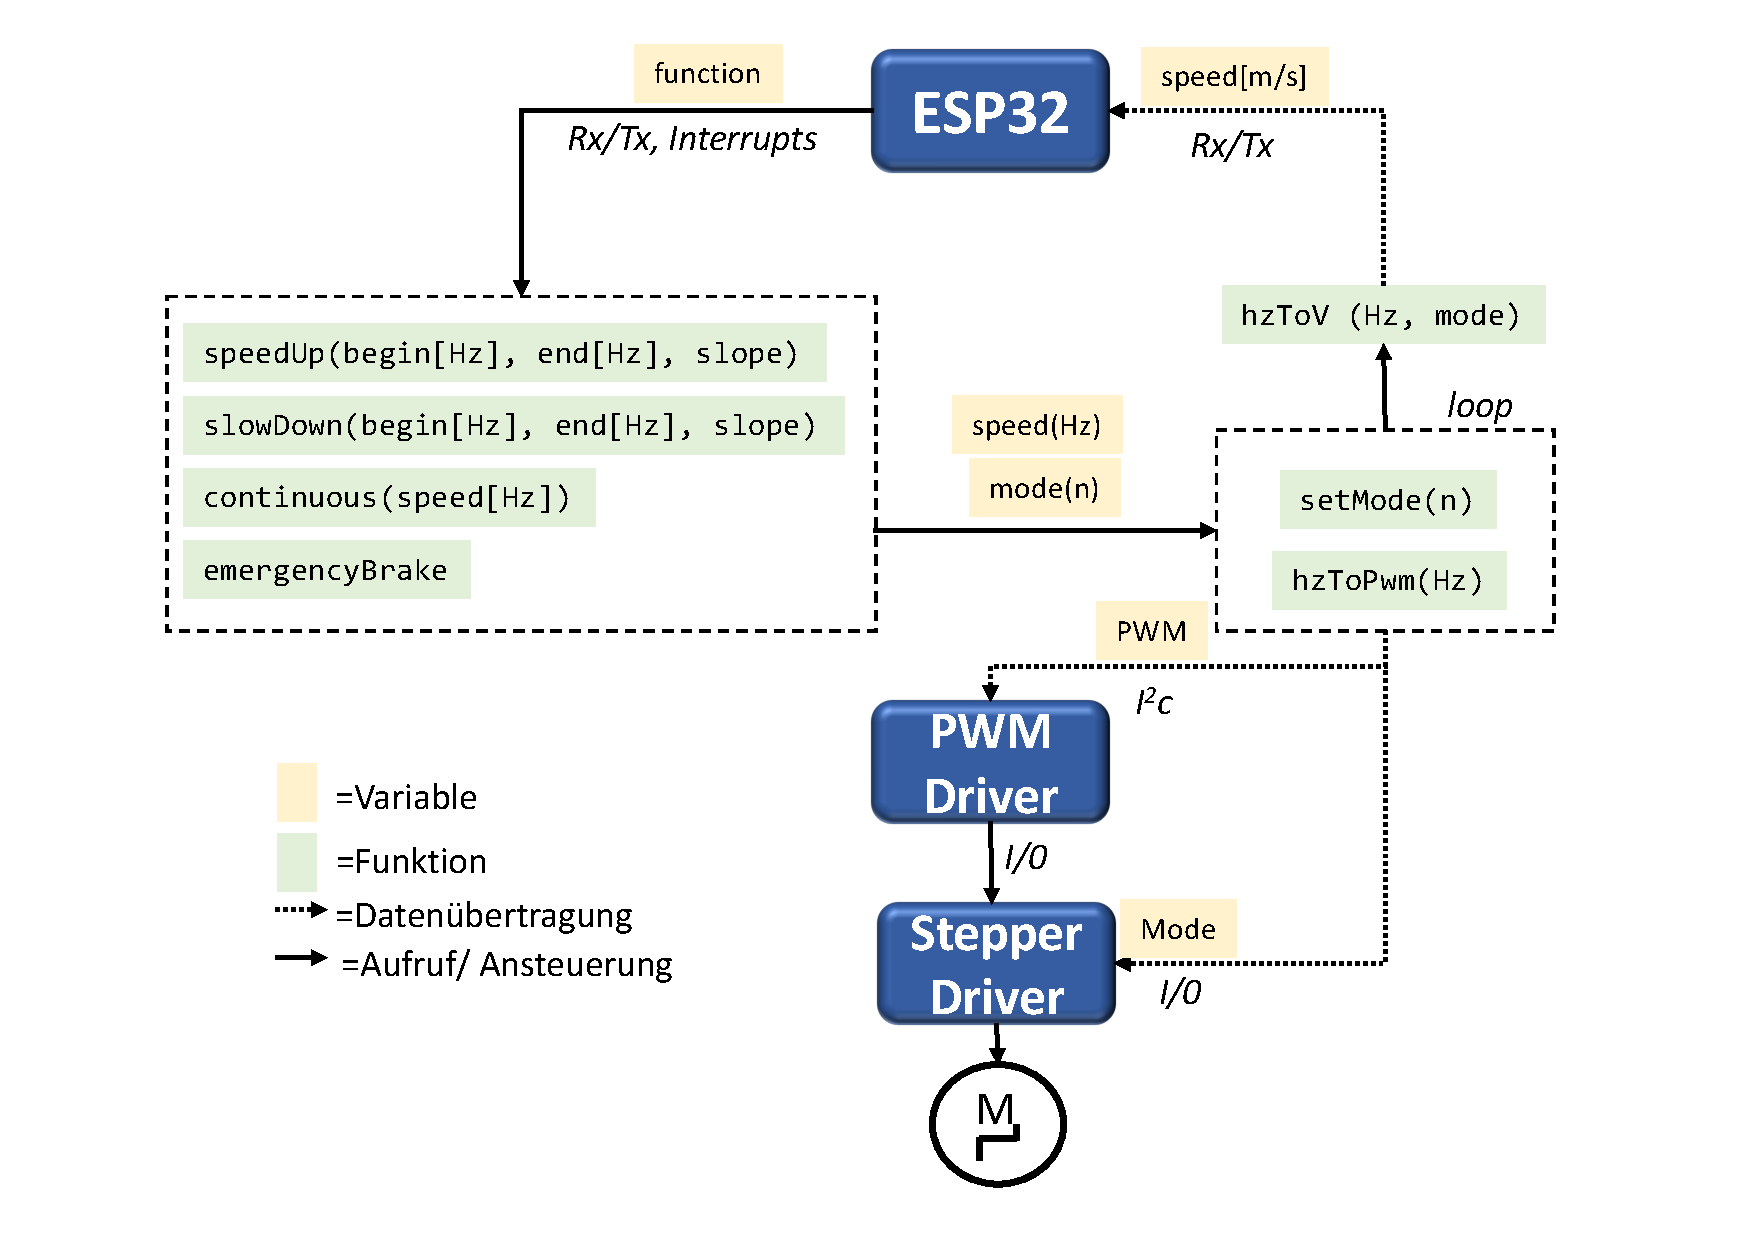
\includegraphics[width=17cm]{motorsteuerung.pdf}
		\caption{Schematische Übersicht der Motoransteuerung}
		\label{pic:motorsteuerung}
	\end{center}
\end{figure}

\newpage

Für die Motorsteueurung können vom ESP32 Funktionen im Skript ausgeführt werden. Für den Brems- und Beschleunigungsvorgang dienen die beiden Funktionen \textit{ speedUp} und \textit{slowDown}. Als Parameter werden die Start- und Enddrehzahl in $Hz$ sowie der Gradient mitgegeben. Bei einer Fahrt mit gleichbleibender Geschwindigkeit wird \textit{continuos} mit Drehzahlparameter in $Hz$ ausgeführt. Wird das Schutzfeld verletzt, löst der ESP32 die \textit{emergencyBrake} Funktion aus. Die Befehle werden über serielle Kommunikation (Rx/ Tx) versendet. Der Nothalt wird durch einen Interrupt am Arduino Nano ausgelöst. \\

Im Skript sind die beiden Variabeln Drehzahl $speed$ und Schrittmodus' $mode$ global angelegt. Diese werden von den Steuerungsfunktionen verändert. Die Variablen dienen den Fukntionen $setMode, hzToPwm$ und $hzToV$ als Grundlage. Diese werden in einer Schleife ausgeführt. $setMode$ stellt den Schrittmodus am Motortreiber über die \acrshort{gpio}-Pins am  Treiber ein. $hzToPwm$ berechnet anhand der aktuellen Drehzahl die Geschwindigkeit in $\frac{m}{s}$. Der Wert wird über die serielle Schnittstelle an den ESP32 zurückgegeben. Die Funktion $hzToPWM$ bestimmt aufgrund der geforderten Drehzahl den \acrshort{pwm}-Wert. Der Wert wird über $I^2C$ an einen  \acrshort{pwm}-Treiber übergeben und dient als Takt für den Schrittmotortreiber. \\

Während ersten Versuchen wurde der Takt für den Schrittmotortreiber vom Mikrocontroller generiert. Dabei zeigte sich, dass die maximale Taktrate stark von der Auslastung des Mikrocontrollers abhängig ist. Durch Verwendung des \acrshort{pwm}-Treibers wird die Takterzeugung ausgelagert. 
 

\section{Getriebekonstruktion}
Wie im Konzeptionierungsteil \ref{sec:getriebekonzept} beschrieben, soll für die Kraftübertragung des Motors auf die Schiene ein Riemengetriebe verwendet werden. In diesem Kapitel wird die Konstruktion des Getriebes beschrieben. In \autoref{pic:getriebe} ist eine Übersicht des Getriebes dargestellt. Auf die Bauteile wird nachfolgend genauer eingegangen. 

\begin{figure}[h]
	\begin{center}
		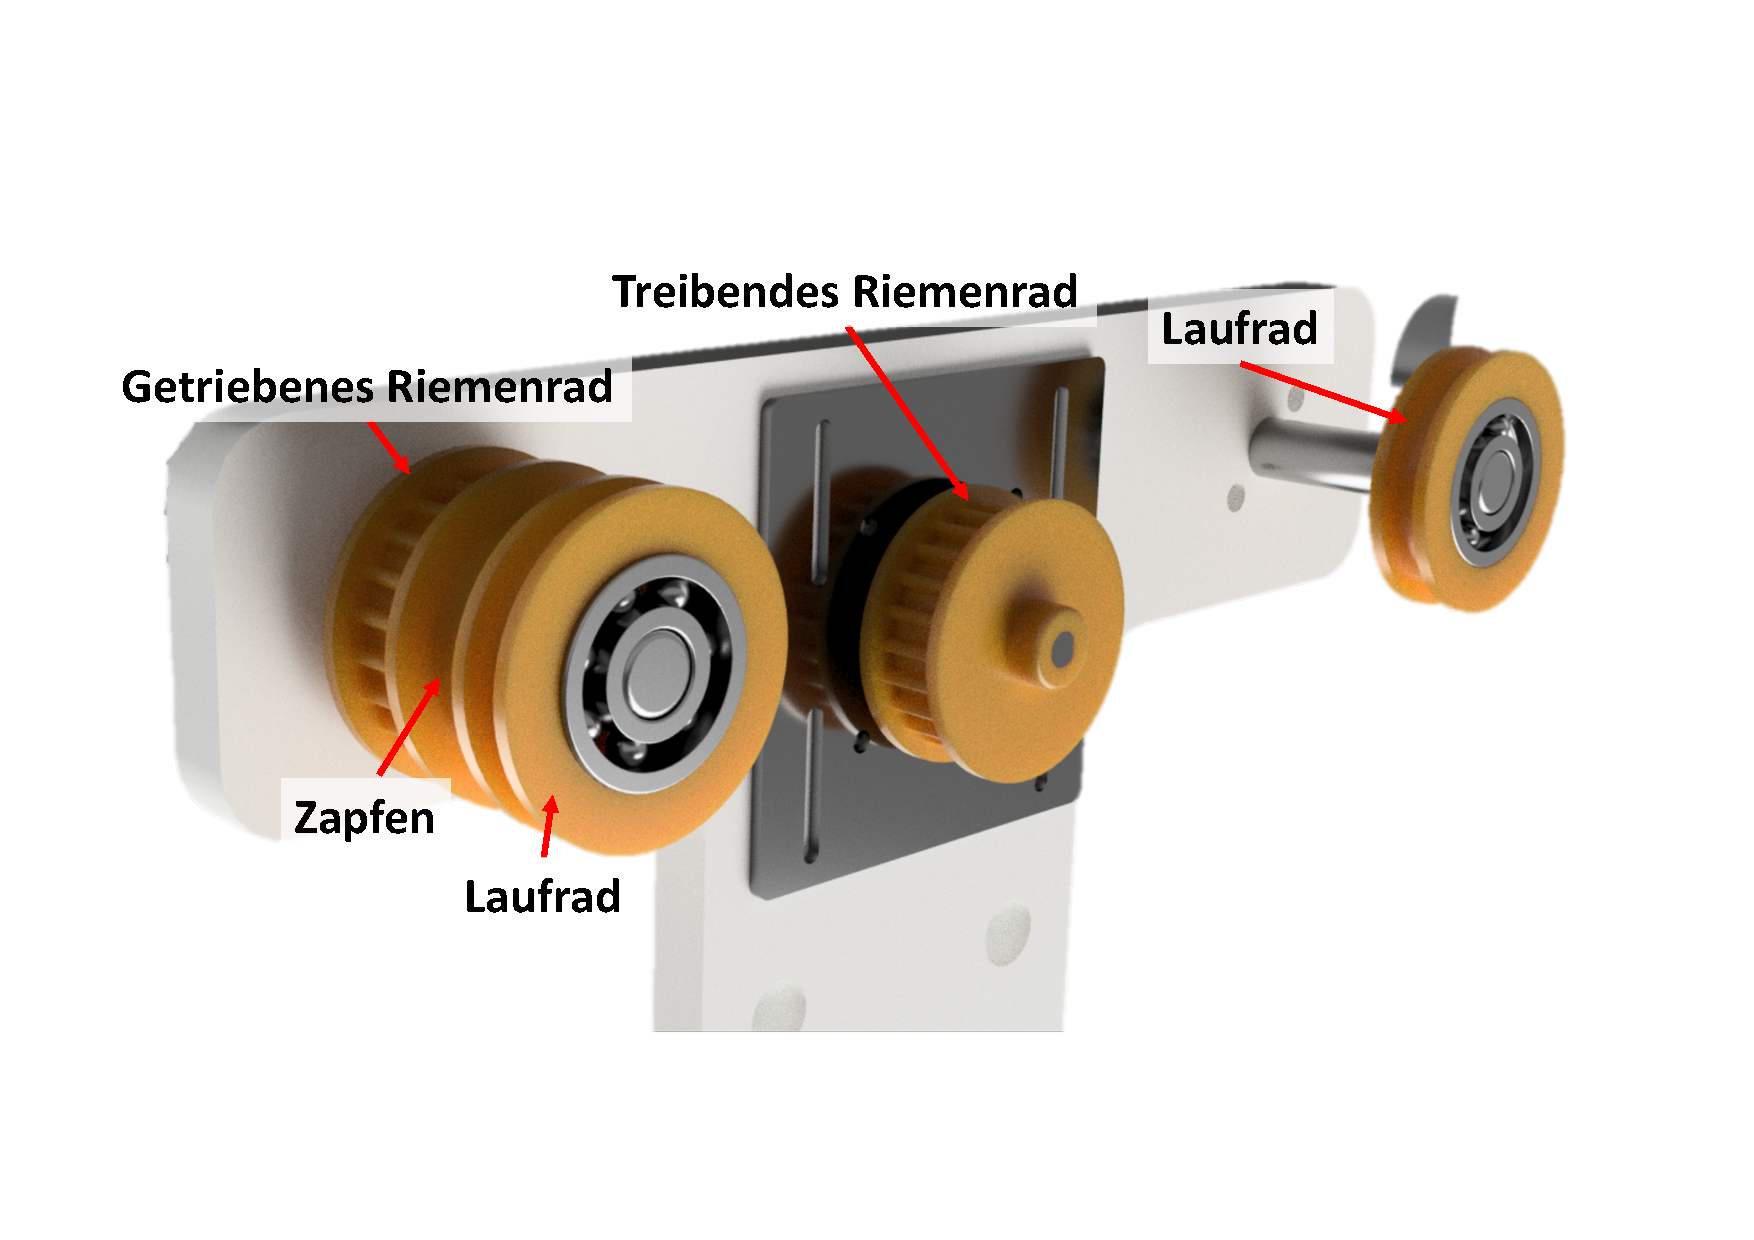
\includegraphics[width=12cm]{getriebe.pdf}
		\caption{Gerenderte Konstruktionsansicht der Getriebekonsruktion}
		\label{pic:getriebe}
	\end{center}
\end{figure} 
\newpage


\underline{Das Laufrad}\\
Beim Laufrad beträgt der Durchmesser der Lauffläche $d=34mm$ bei einer Breite $b=5mm$. Für die Führung auf der Schiene sorgen seitliche Ränder. Diese besitzen eine Breite $b_R=2mm$ sowie einen Durchmesser $d=40mm$. Die Laufräder werden mit einem Rillenkugellager 6000 Welle gelagert. Das Lager wird mit Übermaßpassung verbaut. Das Laufrad ist in \autoref{pic:laufrad}dargestellt. \\

\begin{figure}[h]
	\centering
	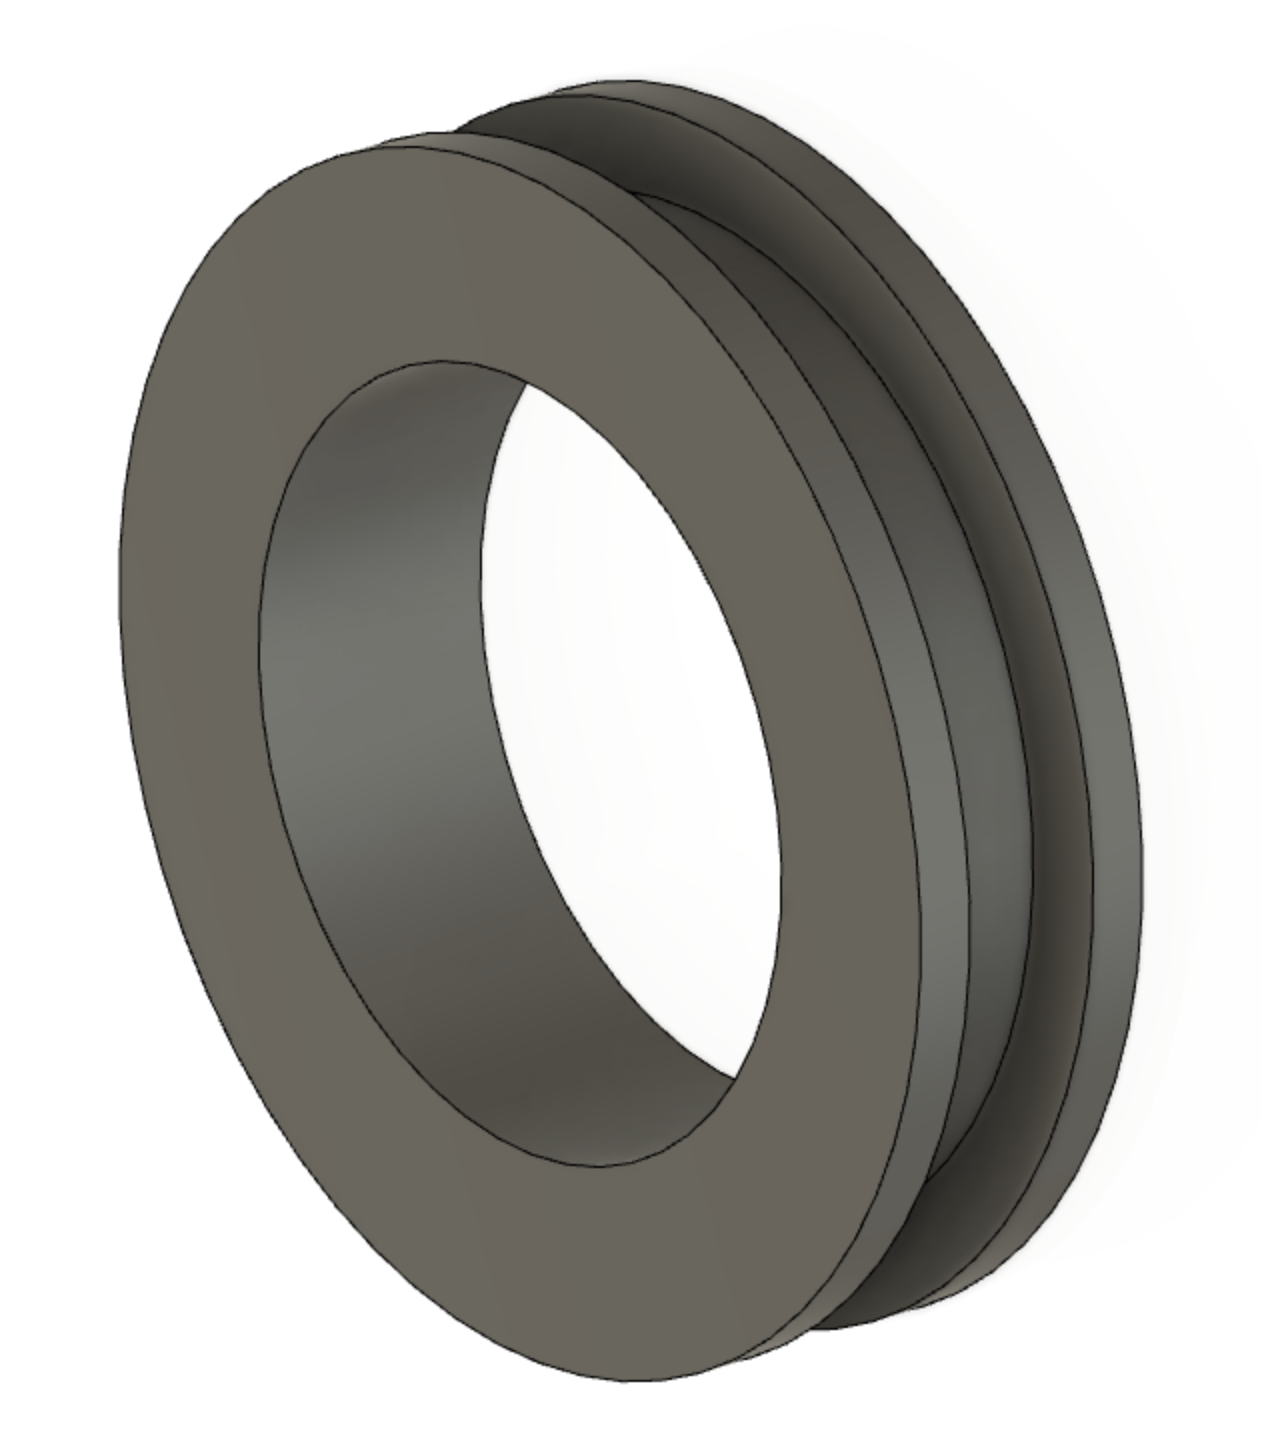
\includegraphics[width=3cm]{laufrad.png}
	\caption{Konstruktionsansicht des Laufrades}
	\label{pic:laufrad}
\end{figure}

\underline{Riemenräder}\\   
Das Riemengetriebe besteht aus einem treibenden und getriebenen Riemenrad. Zunächst soll das Zahnprofil der beiden Riemenräder ausgelegt werden. Dafür ist die Grundlage der Zahnflachriemen mit einem äußeren Umfang von $U = 206mm$ und einer Riemenbreite von $b=9,5mm$. Die Zähnezahl des Riemens beträgt $z_R=75$. Folglich ist das Modul $m \approx 5$. \\

 Für das Zahnprofil muss ebenfalls das Moduel $m=5$ verwendet werden. Die Zähnezahl wird auf $z=22$ festgelegt. Dadurch ergibt sich für den Kopfkreisdurchmesser $d_Z$ des Profils: 
 
 \begin{align}
 	d_Z =  \frac{m \cdot z}{\pi} = \frac{5 \cdot 22}{\pi} \approx 31,05 
 \end{align}


Entsprechend der Abmessungen des Riemens wurde der Durchmesser der Zahnflanken auf 2mm festgelegt.  Das treibende Riemenrad (Ritzel) ist in \autoref{pic:ritzel} dargestellt. Es wird auf die Nabe des Motors gesteckt. Durch die Phase af der Motorwelle geschieht die Übertragung des Drehmoments formschlüssig.  Das getriebene Riemenrad zeigt \autoref{pic:riemenlaufrad} und wird beidseitig gelagert. Dafür wird ebenfalls das Kugellager 6000 mit Übermaßpassung verbaut.  
 

\begin{figure}[h]
	\centering
	\begin{minipage}[t]{0.45\linewidth}
		\centering
		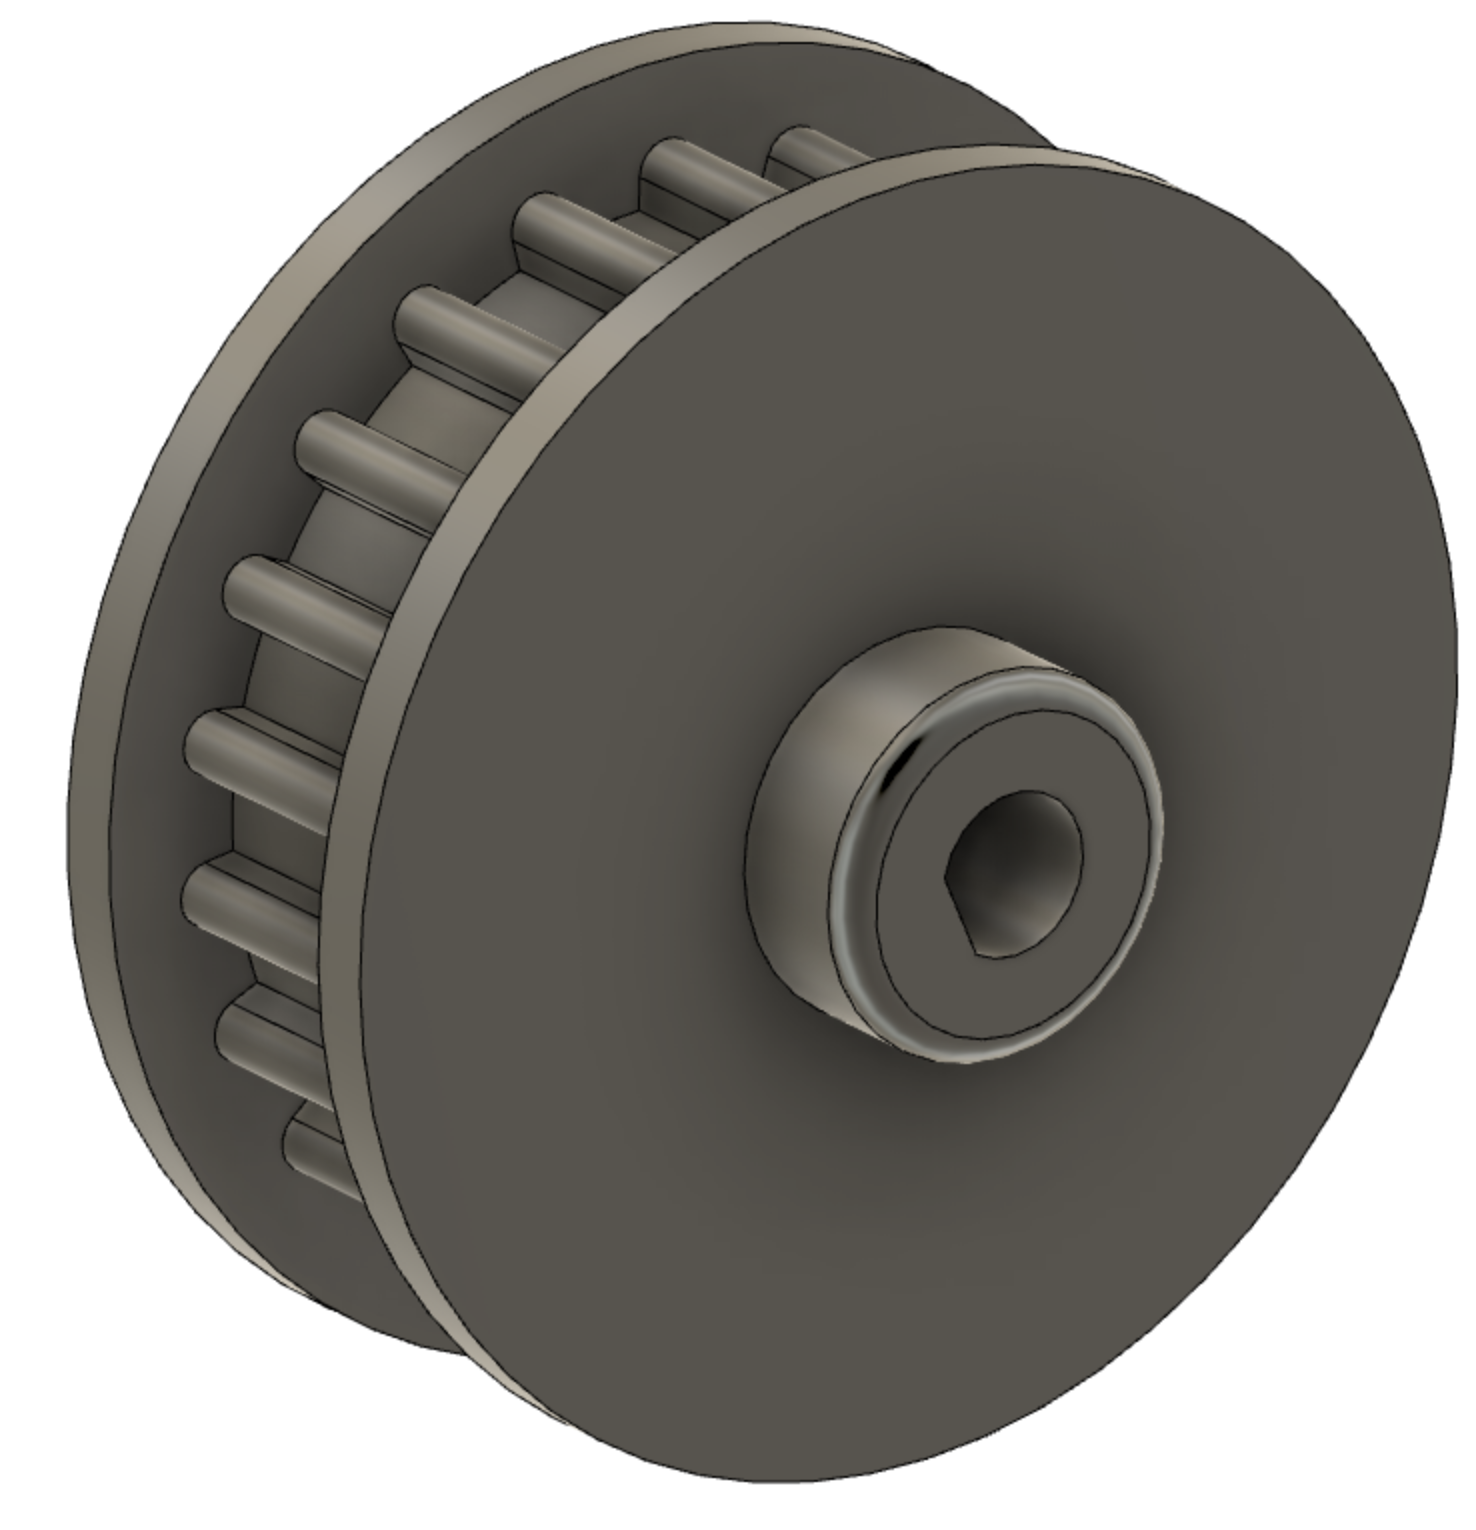
\includegraphics[width=4cm]{ritzel.png}
		\caption{Konstruktion des treibenden Riemenrades (Ritzel)}
		\label{pic:ritzel}
	\end{minipage}
	\hfil	
	\begin{minipage}[t]{0.45\linewidth}
		\centering
		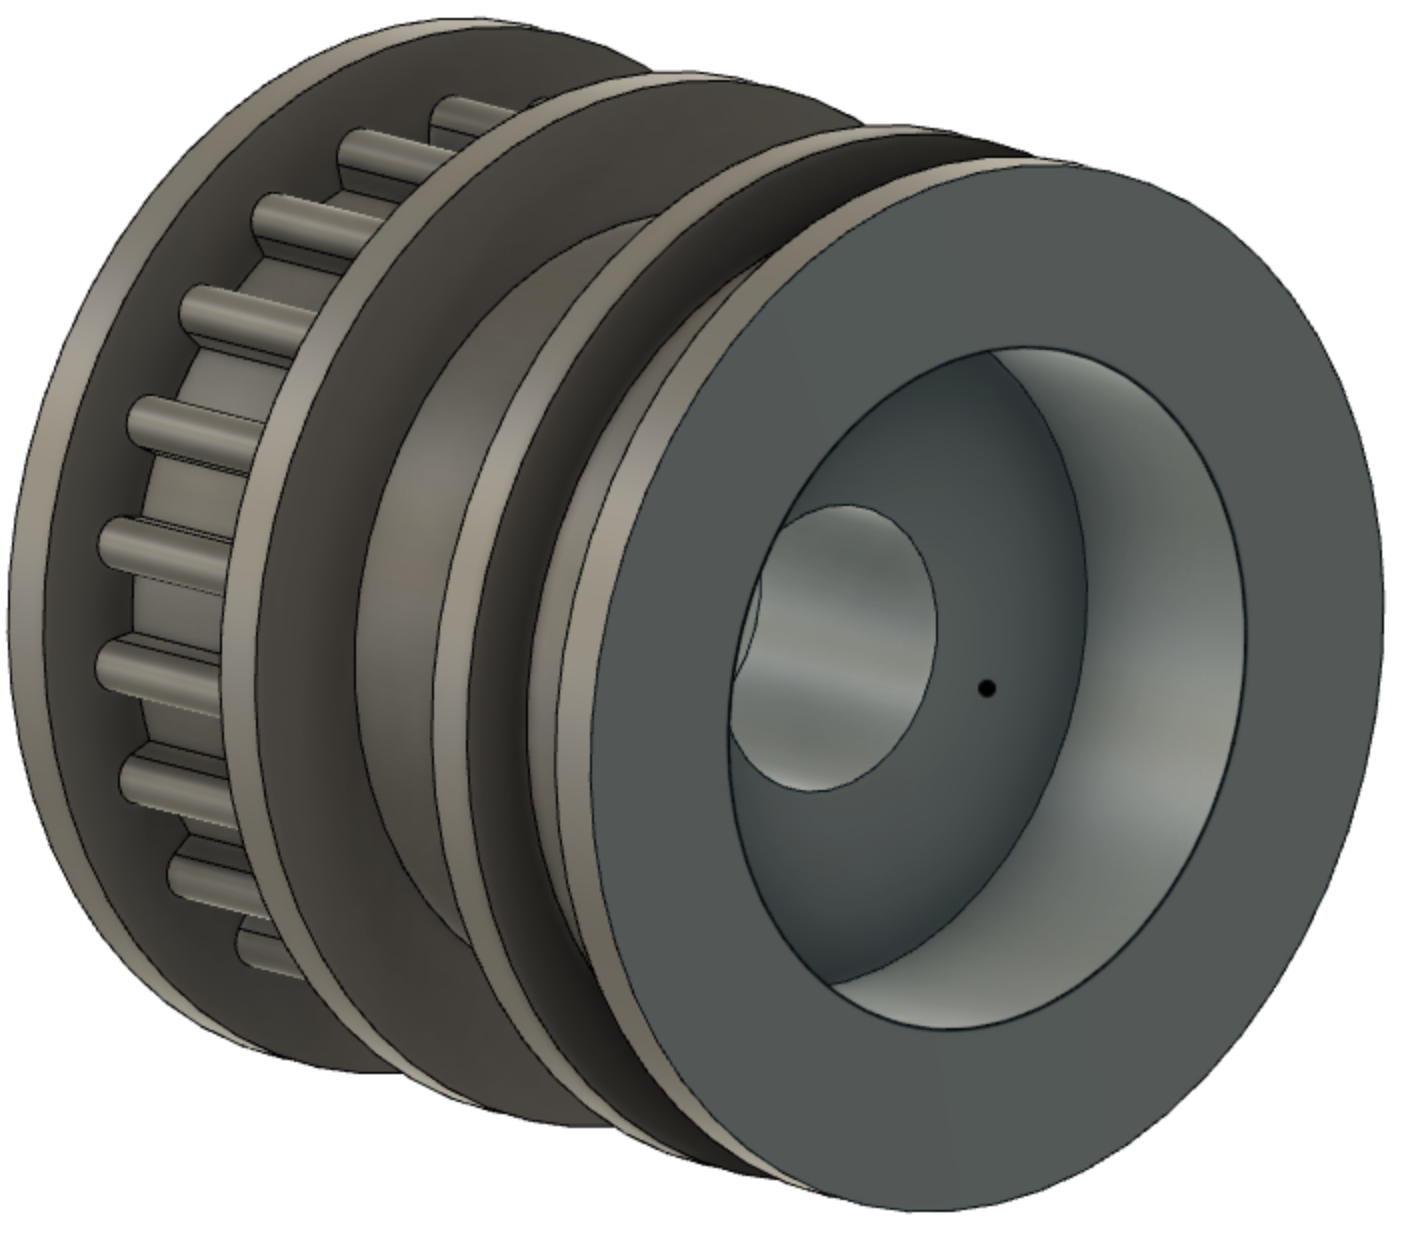
\includegraphics[width=4cm]{riemenlaufrad.png}
		\caption{Konstruktion des getriebenen Riemenrades mit Laufrad}
		\label{pic:riemenlaufrad}
	\end{minipage}	
\end{figure}



\newpage


\underline{Implementierung des Getriebes}\\
Der äußere Umfang des Riemens beträgt $U = 206mm$. Für die Berechnung des erforderlichen Abstandes $\Delta$ der beiden Wellen zueinander gilt mit dem Riemenraddurchmesser $r$ folgende Formel: 


\begin{align}
	U = 2 (r+ \Delta) \\
	\Delta = \frac{U - 2r}{2} = \frac{206mm - 35,01}{2} \approx 85mm 
\end{align}

Um den Wellenabstand zu erreichen, wird die Motoraufhängung nach unten entsprechend versetzt. Zusätzlich soll sich die Aufhängung nach der Montage in Y-Richtung justieren lassen. Dadurch kann der Riemen nach dem Einbau auf Spannung gebracht werden. Die Motoraufhängung ist in \autoref{pic:motoraufhaengung} dargestellt. 


\begin{figure}[h]
	\centering
	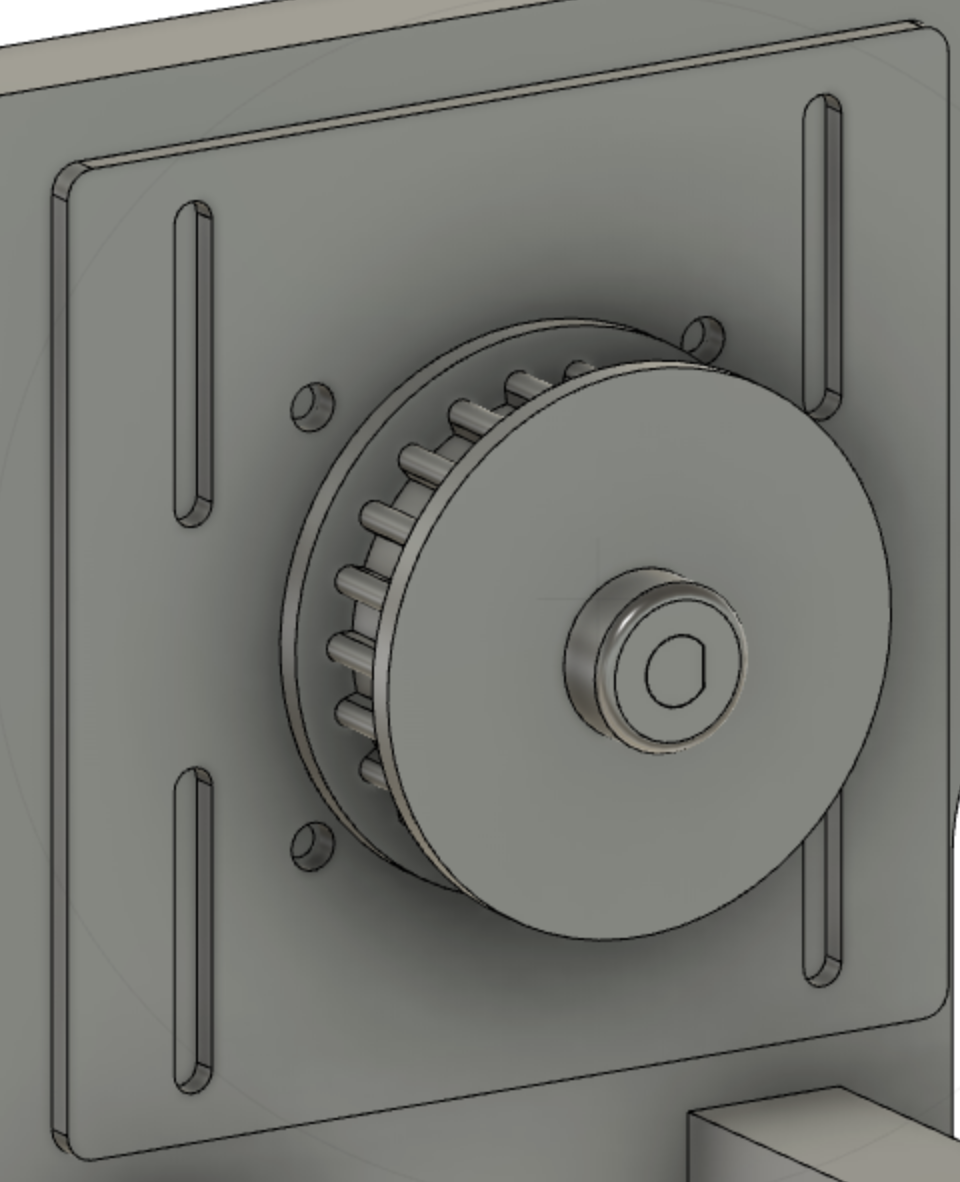
\includegraphics[width=5cm]{motoraufhaengung.png}
	\caption{Konstruktionsansicht der verschiebbaren Motoraufhängung}
	\label{pic:motoraufhaengung}
\end{figure}

Die Wellen werden axial beansprucht. Damit die Befestigung der Welle die axialen Kräfte aufnehmen kann, wird zusätzlich ein Rundmaterial an die Seitenteile montiert. 


\section{Fertigungsverfahren}
Für 
Für die vorgestellten Bauteile soll nun das Fertigungsverfahren ausgewählt weden. Dabei besteht die Möglichkeit konventionelle- und adaptiven Fertigungsverfahren zur Auswahl.


\begin{figure}[h]
	\centering
	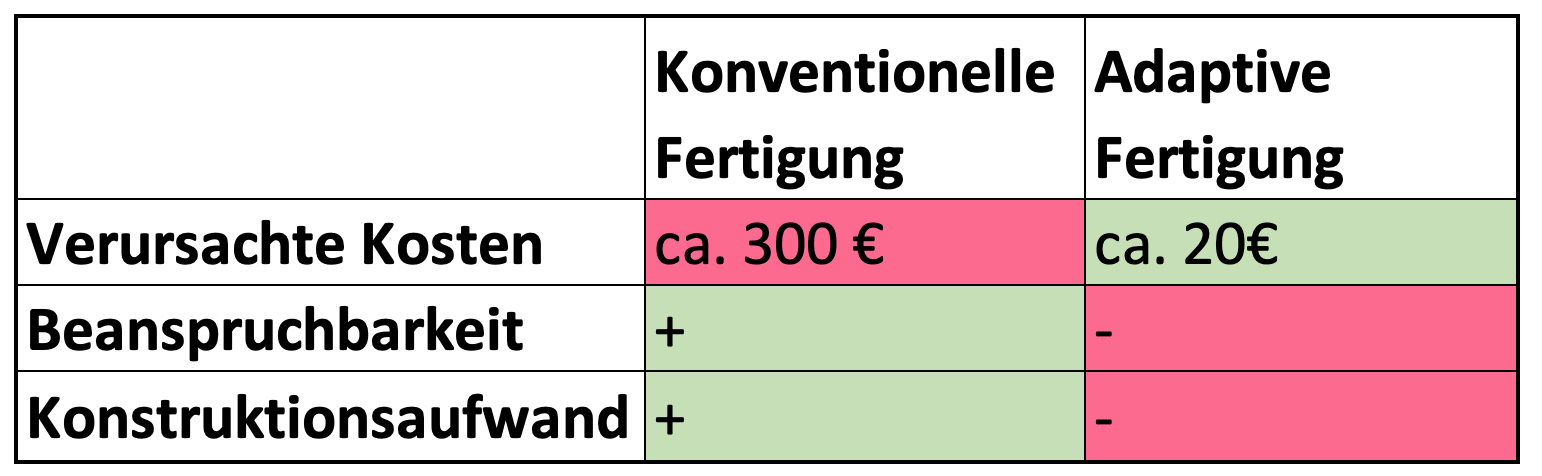
\includegraphics[width=12cm]{fertigungsverfahren.png}
	\caption{Konstruktionsansicht der verschiebbaren Motoraufhängung}
	\label{pic:fertigungsverfahren}
\end{figure}


Aufbereitungs-  Rüstzeit 

Bei hoch beanspruchten Teilen: Konventionelle Fertigungsverfahren 
Aufwändige Konturen: Adaptive Fertigung


	
    \chapter{Diskussion und Ausblick}

\lipsum
\end{onehalfspace}

\clearpage
\pagenumbering{roman}
\setcounter{page}{4}
\appendix

% bibliography
\printbibliography[title={Literaturverzeichnis}]
\addcontentsline{toc}{chapter}{Literaturverzeichnis}

% list of abbreviations, glossary of terms
\printglossary[title={Abkürzungsverzeichnis},type=\acronymtype]
\printglossary

\end{document}